\documentclass{mproj}
\usepackage{graphicx}
\usepackage{subcaption}
\usepackage{subfig}
\usepackage{graphicx}
\usepackage{url}
\usepackage{fancyvrb}
\usepackage[final]{pdfpages}
\usepackage{subfloat}
\usepackage{floatrow}
\usepackage{wrapfig}
\usepackage{picinpar}
\usepackage{fancyref}
\usepackage{amsmath}
\usepackage{listings}
\usepackage[font=scriptsize]{caption}
\lstdefinestyle{customc}{
basicstyle=\footnotesize,
numbers=left,
keywordstyle=\bfseries\color{orange},
commentstyle=\itshape\color{purple!40!black},
stringstyle=\color{green!40!black},
}
\lstset{escapechar=@,style=customc}



\graphicspath{{images/}}

% alternative font if you prefer
\renewcommand{\familydefault}{\sfdefault}
\usepackage{helvet}
\usepackage[T1]{fontenc}
\usepackage{textcomp}

% for alternative page numbering use the following package
% and see documentation for commands
%\usepackage{fancyheadings}


% other potentially useful packages
%\uspackage{amssymb,amsmath}
%\usepackage{url}
%\usepackage{fancyvrb}
%\usepackage[final]{pdfpages}

\begin{document}

%%%%%%%%%%%%%%%%%%%%%%%%%%%%%%%%%%%%%%%%%%%%%%%%%%%%%%%%%%%%%%%%%%%
\title{Gold Digger: a metaphor for searching behavior}
\author{Gabriele Giordano Maria Rossi}
\date{08/09/2014}
\maketitle
%%%%%%%%%%%%%%%%%%%%%%%%%%%%%%%%%%%%%%%%%%%%%%%%%%%%%%%%%%%%%%%%%%%

%%%%%%%%%%%%%%%%%%%%%%%%%%%%%%%%%%%%%%%%%%%%%%%%%%%%%%%%%%%%%%%%%%%
\begin{abstract}
In this paper we set out to investigate if expectations about user searching behaviour raised by the Optimal Foraging Theory can be met in an environment that \textit{simulates} scenarios that would require decisions and
actions we would have to make while looking or informations.

The environment chosen is a game: Gold Digger. In this game users can dig through mines and acquire gold, as a metaphor for searching and acquiring useful information. Users were able to play this game as they pleased, with no instructions as to what the optimal behaviour should be.A total of 39 users/players enterd the experiment/game over a three week period.

At the end of this period, our findings seem to match expectations. Users move from one mine to the other when the first one stops being productive at the right time with an absolute discrepancy of only one layer. 

\end{abstract}
%%%%%%%%%%%%%%%%%%%%%%%%%%%%%%%%%%%%%%%%%%%%%%%%%%%%%%%%%%%%%%%%%%%

%%%%%%%%%%%%%%%%%%%%%%%%%%%%%%%%%%%%%%%%%%%%%%%%%%%%%%%%%%%%%%%%%%%
\educationalconsent

%%%%%%%%%%%%%%%%%%%%%%%%%%%%%%%%%%%%%%%%%%%%%%%%%%%%%%%%%%%%%%%%%%%

\newpage
%%%%%%%%%%%%%%%%%%%%%%%%%%%%%%%%%%%%%%%%%%%%%%%%%%%%%%%%%%%%%%%%%%%
\section*{Acknowledgements}

Firstly, I would like to thank Leif Azzopardi, our project leader and supevisor, for his expertise, insight and advice throughout the development of this project and during the project proposal. 

I also would like to thank David Maxwell and Sean McKeown for their patience, feedback and the amount of time they took to help us develop Gold Digger.

Finally, I would like to thank all of the users who played Gold Digger and in particular Martin Crean for his advice on game features and Martyna Mar�n. 

%%%%%%%%%%%%%%%%%%%%%%%%%%%%%%%%%%%%%%%%%%%%%%%%%%%%%%%%%%%%%%%%%%%
\tableofcontents


%%%%%%%%%%%%%%%%%%%%%%%%%%%%%%%%%%%%%%%%%%%%%%%%%%%%%%%%%%%%%%%%%%%
\chapter{Introduction}\label{intro}

\section{Overview}

Information management is becoming an essential part of our professional and personal lives. Whether it is in order to write a report, to do research, or simply to look for inspiration, we often turn to the internet, and increasingly less to paper-based media, to search for the information we need.
Yet, to be able to make use of the vast resources at our disposal, it is increasingly important to be effective in finding ways to shorten the time spent searching, while maximising the amount of useful information found, or the 'rate of gain'.
The aim of this project was therefore to provide insights into the strategies users apply to search for information and shed light on how they make searching more effective. There are however many different parameters that influence our rate of success when searching for information, such as our familiarity with the kind of information we are searching for, and our skill in using the searching tools themselves.
The challenge and main objective of this project was to create a context in which all users can have the same starting conditions irrespective of pre-existing abilities, and subsequently analyse and investigate their searching behaviour. 

To this purpose, we designed a game that would serve as environment to investigate searching behaviour while being abstracted from any potentially biasing context. This game, Gold Digger, simulates the actions and decisions users would face while searching for information, but not actually present them with an information retrieval task.
This way, the game would make it possible to put users on the same starting point, since previous insight on information retrieval would not be applicable. As an experimental platform, it allows easy modification of its parameters and could therefore be used to carry out multiple experiments with different focus. In addition to this, the game also presents a familiar environment to users where they can have fun and will be motivated to use the system over a long time.  

In Gold Digger, searching is represented by entering a mine. Examining one of the pieces of information we find and thereby acquiring useful information, is represented by digging and obtaining gold. The amount of gold that the player is able to extract from a given mine, is determined by their ability to decide whether the mine is still profitable to dig in or if it is better to move to a new mine instead, much in the same way we would decide to examine the list of links returned by a search engine one by one, or enter a new query instead. Because digging and moving both have a cost in time units, the player will need to find the most profitable way to act before the end of the day. Entering a mine also has a cost, so players will need to make sure to acquire enough gold before the end of one day to be able to continue mining. 
Players can purchase a variety of items that will allow them to gain more gold, dig or move at a lower cost or even be able to get clues on the profitability to dig in a mine. These items represent the 'enrichment strategies� we use while looking for information, for instance having different tabs open on a browser to quickly flick through different pages. Finally, players are also able to gain special achievements for their performance and be ranked in leaderboards.
Gold Digger is therefore an effective and creative representation of information retrieval that gathers invaluable information to further analyse search behaviour and can easily be adapted to evolving research aims, as well as keeping players engaged and motivated to take part. As a result, a very large amount of (completely anonymised) data on registered users� performance has been generated and is currently being processed. 

Today, the ability to retrieve greater amounts of useful information in smaller amounts of time is becoming an invaluable skill to navigate both our professional and private lives. 
The insights Gold Digger can provide will help to improve information retrieval techniques, to optimise content design, and could make the skills needed to search for, find, manipulate, and make sense of vast amounts of information more accessible. 

\subsection{Problem statement}
This project proposes to analyse user's searching behaviour in a context deprived of any cues 
that could allow them to exploit any previous experience in the task in order to achieve an 
optimal information foraging behaviour. 
User's performance will be recorded and evaluated to see if it matches data in experiments in 
which this context is present. Findings could help provide insight on people's choices when 
faced with a task that requires the same kind of skills that are required in information foraging 
with none of the context that they are presented with in experiments based on the same 
theories.
Finally this project aims at making user's experience as enjoyable as possible for two reasons.
Firstly it will avoid users feeling like they are performing work, removing them further from a 
standard information foraging task. Secondly, in order to enhance the number of users that 
play the game as well as the amount of games played.


%%%%%%%%%%%%%%%%%%%%%%%%%%%%%%%%%%%%%%%%%%%%%%%%%%%%%%%%%%%%%%%%%%%
\chapter{Survey}
\label{ch:survey}

\section{Background theories }

\subsection{Optimal Foraging Theory}
\label{subsec:OFT}
One of the most interesting studies proposed by Sinevro which can help us bring out some interesting points on searching behaviours, is the one on crows foraging on clams. In this study, Sinevro tells us about the foraging behaviour of the common crow (Corvus caurinus) in the intertidal. This kind of crow, has developed a technique to open clams which requires it to take a short flight and drop clams on some rocks below it to crack them open. The cost (in energy) of searching for clams, and the one of handling them is almost the same, however, the cost (in time) of performing the same activities is 4 times more expensive with regards to searching. It is then difficult to understand why crows would reject a large amounts of the clams they find, especially given the fact that searching seems to take up so much time. The reason for this behaviour is to be found in the "average net profitability of the clams as a function of size�(Sinevro 2006), which can be represented by the equation:

\begin{equation*}
\frac{\emph{Energy}}{ \emph{Time}} = \frac {\emph{Energy per clam as a function of size - (Search Cost + Handling Cost)}}{ \emph{(Search Time + Handling Time)}}
\end{equation*}

It is very interesting to notice that predictions on the crow's behaviour in order to maximise energy gain per unit of time according to this formula, closely match its observed behaviour.
\begin{figure}[!h]
        \centering
	\caption{frequency of clams in class size (\% on y axis) by clam length (x axis)}
	\label{fig:clams}
        \begin{subfigure} [h] {0.3\textwidth}
                \centering
                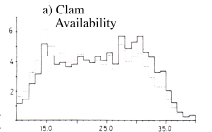
\includegraphics [width=1\textwidth] {clam1.png}
		\caption{}
        \end{subfigure}
        \space
        \space
        \begin{subfigure} [h] {0.3\textwidth}
                \centering
                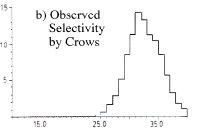
\includegraphics [width=1\textwidth] {clam2.png}
		\caption{}

        \end{subfigure}
	\space
	\space
	\begin{subfigure} [h] {0.3\textwidth}
                \centering
                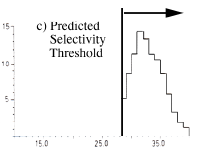
\includegraphics [width=1\textwidth] {clam3.png}
		\caption{}

        \end{subfigure}
\end{figure}

As we can see from (b) and (c) in fig \ref{fig:clams}, predicted behaviour seems to closely match observed behaviour. This kind of model, however, considers the disposition of prey in the environment to be random but, sometimes, prey items seem to have a patchy distribution (Sinevro 2006). In this case, an animal will have to travel between patches before it can start exploiting a new one. This creates two variables according to which an animal has to "make its decision" in order to maximise its rate of gain. The first one is the time spent within a patch to feed, and the second one is the time spent travelling between patches in which, crucially, the animal doesn't gain any energy and instead consumes it. A formula that effectively models this choice is:

\begin{equation*}
\emph{Rate of energy gain} = \frac{\emph{Energy}}{ \emph{Time}} = \frac {\emph{Energy or Load Size}}{ \emph{(Travel time to patch + Foraging time to patch}}
\end{equation*}

Also known as "\textbf{Charnov's Marginal Value Theorem}" which generates an energy gain function like the one on the left. Here, we can see how there are two main areas delimiting the Cartesian space, the first one (on the left side of the curve) is the potential time the animal has to spend in between patches, whereas the second one is the potential time spent feeding in a single patch. An optimal allocation of time in foraging for this rate of gain will be represented by the tangent to the curve as shown in the graphs on the right. The red line is the tangent and the point of intersection with the curve determines the in-patch time that would be optimal for an animal to spend feeding.

\begin{figure} [!ht] 
	\centering
           \makebox[\textwidth][c]{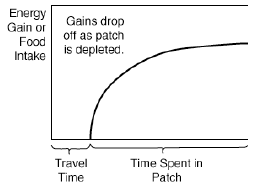
\includegraphics[width=0.4\textwidth]{gain1.png}}
	\caption{An energy gain function}
           \label{gain1}
\end{figure}

The aim of this proposal is evaluate subjects' innate ability to reproduce similar behaviours while foraging for information rather than for food. To do this, the context of a gold digging strategy game has been chosen, in order to remove all proximal cues that might depend on the user's previous experience. In this environment, the user will have to perform the same kind of cost vs. benefit choices, however, he would not be able to adopt the strategies he consciously would. Following I discuss a paper by Pirolli \& Card on Information Foraging which seems to support this intuition proposing experimental evidence and mathematical models.  "

\begin{figure}[!h]
        \centering
	\caption {The optimal rate of gain}
	\label{fig:gain tangent}
        \begin{subfigure} [h] {0.49\textwidth}
                \centering
                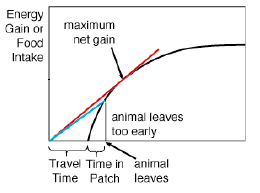
\includegraphics [width=1\textwidth] {gain2.png}
        \end{subfigure}
        \space
        \space
        \begin{subfigure} [h] {0.49\textwidth}
                \centering
                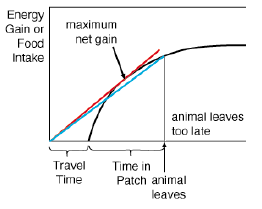
\includegraphics [width=1\textwidth] {gain3.png}
        \end{subfigure}
\end{figure}

\subsection{Information Foraging Theory}
\label{subsec:IFT}
Pirolli \& Card seem to start from the assumption that there are many similarities between the techniques adopted by animals foraging in the wild and the ones adopted by people in "Information Foraging". Because of the structure of today's society, in fact, it is not for food that we forage for. Food is usually readily available almost anywhere  human settlements can be found, however, to purchase it, we need to engage in a "complex tributary of cultural tasks that engage our physical and social environments" (Pirolli \& Card  1995) which demand us to develop numerous "information-based" strategies, in order to earn a living. Pirolli \& Card begin by explaining that our adaptive success seems to be increasingly dependent on our mastery of techniques of information-gathering, sense-making, decision-making and problem-solving strategies. In turn, they claim, this leads us to implement strategies which are similar to the ones seen in foraging behaviours of animals in the wild. Here, we can observe patterns in food foraging behaviours which aim at maximising the energy intake while minimising the amount of energy spent while foraging. 

In other words, our lives are increasingly dependent on the ways in which we organise and retrieve information in order to use it effectively to navigate and survive today's social (and sometimes physical) landscape. Pirolli \& Card go on to claim that, the Information Foraging theory's main tenant is that:  "when feasible, natural information systems evolve towards stable states that maximise gains of valuable information per unit cost. Cognitive systems engaged in information foraging will exhibit such adaptive tendencies" (Pirolli \& Card  1995). 

As a consequence, it is to be expected that people will modify their information foraging strategies as well as the structure of the environment itself, whenever possible, to "maximise the rate of gaining valuable information" (Pirolli \& Card  1995). Better strategies will be the ones that will allow someone who adopts them to yield more information per unit cost. Furthermore, it is also expected that these strategies will evolve through time, in order to reach a seemingly stable state that maximises the potential gains. 

The process of analysing the development of this kind of behaviour, is called "adaptation analysis". This kind of analysis is conducted here, as well as in biology, through the use of "optimisation models" to study the design features of organisms and artefacts. Optimisation models include three major components:

\begin{itemize}
	\item \textit{Decision assumption}, determine how much time is to be spend analysing a certain collection of information as well as which kind of content is worthwhile pursuing.
  	\item \textit{Currency assumptions}, determine how the choices made through decision assumptions are to be evaluated. In the context of Information Foraging, the relevant currency will be amount of relevant documents found, as opposed to the amount of energy gained in food foraging strategies.
  	\item \textit{Constraint assumptions}, determine what kind of limits will apply to the relationship between decision and currency assumptions. In Information Foraging, these include (but are not limited to) previous knowledge, available technology and task structure.
\end{itemize} 

These models allow us to construct a framework for the evaluation in Information Foraging, however, it is not to be expected that any single individual will fully be conscious and even evolve towards, an optimal awareness and implementation of these models. These models simply outline the possibility of "an advantageous adaptation if not blocked by other forces. 

The main decision an organism has to make in its foraging endeavours (being it for food or for information) is determined by a problem of "Enrichment vs. Exploitation� of a certain "patch of relevant documents (or food). The careful weighing of one against the other, will, in turn, determine its searching behaviour, comprehensive of "in-patch� and "between-patch behaviours.  When we decide to "enrich� a certain patch of information, we engage in certain "enrichment strategies� which are meant to maximise the amount of relevant information per unit of cost that we are able to get from a patch. However, the adoption of these strategies themselves has a cost which should be considered when making the decision to move to a different patch and select a new set of documents. There are two main "in-patch� enrichment strategies. 

The first one is based on producing information packages that yield better results. This involves strategies like developing or acquiring better search tools, as well as spending time mastering them. The second one is based on filtering the incoming information into relevant topics or according to other decisional criteria devised by the foragers and that they came to realise as useful to their foraging needs. 

Another way foragers can increase their gain in yielded by their foraging behaviours is by using "between-patch� enrichment strategies. These are also of two kinds. The first one is constituted by what Pirolli \& Card call "scent-detection strategies�. These strategies are based on the identification of proximal cues in the environment in order to make a choice on whether it would be fruitful to explore a certain "patch� or move to another one based on detection of proximal cues. In the context studied by Pirolli \& Card, this translates into identifying the relevance of a certain document, or group of documents by, for instance, its title and payoff, perceived clarity of writing or length. 

A second kind of in-patch enrichment strategy is based on reducing the cost of getting from one information patch to another. While this is usually impossible for animals in the wild, because it involves modifying the environment, it is instead a very efficient way for information foragers to improve the rate of gain per unit cost. In the example proposed by Pirolli \& Card this is shown in the re-organisation of the workspace of an employee whose job is to write a Business Intelligence Newsletter. The subject of their experiment, in fact, organised the different areas of his office, in order to minimise the time spent searching for relevant document by disposing the material he knew he would need more frequently, the nearest to his working station.

For the purpose of this proposal it is also important to consider the conventional models of foraging on which Information Foraging Theory is based. As it can be expected, to provide an efficient model of foraging, we will have to take into account equations which model both in-patch and within-patch behaviours. Given what previously stated, Pirolli \& Card start by characterising the rate of gain of valuable information per unit cost R as the ratio of the total net amount of valuable information gained $G$ divided by the total amount of time spent between patches $T_B$ and exploiting within patches $T_W$ a

\begin{equation}
R = \frac{G}{T_B + T_W}
\label {eq:main}
\end{equation}

Notably, this equation assumes that (1) "the total amount of information gained can be represented as a linear function of between-patch foraging time:

\begin{equation}
G = \lambda T_B g
\end{equation}

And that (2)�the total amount of within-patch time can be represented as:

\begin{equation}
T_W = \lambda T_B t_W
\end{equation}

This, in turn, gives Holling's Disc Equation:
\begin{equation}
\begin{split}
 R = \frac{\lambda T_B g}{T_B + \lambda T_B t_W} \\
= \frac{\lambda g}{1 + \lambda t_w}
\end{split}
\end{equation}

This formulation, however, "addresses the problem of allocation of time between in-patch vs. between patch under certain strong assumptions". Because of this, Pirolli \& Card have to devise their own interpretation which takes in to account that "(a) there might be different kinds of patches and (b) the total gains from a patch depend on the within-patch foraging time which is under the control of the forager. For this reason they have to include a value \emph{i} representing the type of patches encountered at a rate of $\lambda$ i and a value $t_wi$ representing the \emph {policy} adopted by a forager on how much time to spend within each patch. The total gain can then be represented as the sum of all the values of \emph{i} between 1 and P.

\begin{equation}
\begin{split}
G = \sum_{\substack{i=1}} \lambda_i T_B g_i (t_{wi}) \\
= T_B  \sum_{\substack{i=1}} \lambda_i g_i (t_{wi})
\end{split}
\end{equation}

In the same way, the total amount of time spent within patches could be represented as:

\begin{equation}
\begin{split}
T_W = \sum_{\substack{i=1}} \lambda_i T_B t_{wi} \\
= T_B  \sum_{\substack{i=1}} \lambda_i (t_{wi})
\end{split}
\end{equation}

Combining these two equations according to (eq. \ref{eq:main}) gives us:

\begin{equation}
\begin{split}
R = \frac{T_B \sum_{\substack{i=1}} \lambda_i g_i (t_{wi})}{T_B + T_B  \sum_{\substack{i=1}} \lambda_i t_{wi} } \\
= \frac{\sum_{\substack{i=1}} \lambda_i g_i (t_{wi})}{1 + \sum_{\substack{i=1}} \lambda_i t_{wi} }
\end{split}
\end{equation}

This last equation is what Pirolli \& Card call the \emph"patch model for information foraging" which takes into account patches that yield different kinds of gain functions as well as different strategies to exploit them.

\begin{figure} [!ht] 
	\centering
           \makebox[\textwidth][c]{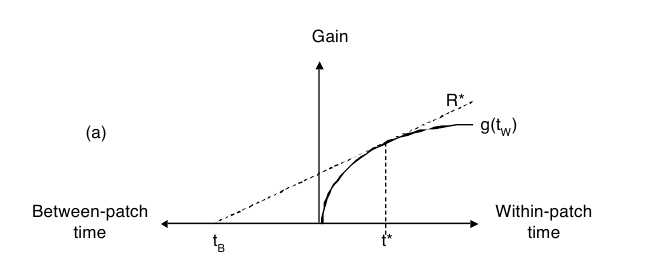
\includegraphics[width=0.8\textwidth]{enrichment1.png}}
	\caption{(a) - The Graph illustrates Charnov's Marginal Value Theorem  where t* denotes the optimal amount of time spent within-patch given the intersection between the gain function $g(t_w)$and the tangent passing from $t_B$ (the time spent between patches)}
           \label{gain1}
\end{figure}
\begin{figure} [!ht] 
	\centering
           \makebox[\textwidth][c]{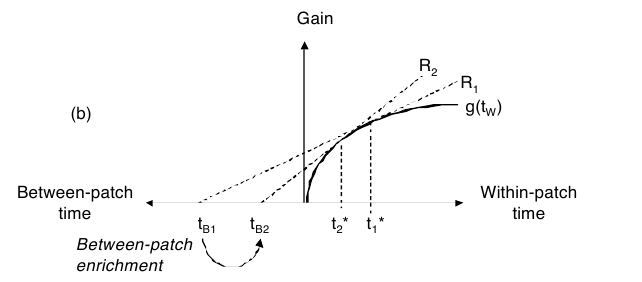
\includegraphics[width=0.8\textwidth]{enrichment2.png}}
	\caption{(b) - Shows the changes generated by the adoption of between-patch enrichment strategies. The tangent to the gain function $g(t_w)$ passing from $t_{B2}$  determines that the optimal amount of time to spend in a given patch is now $t_2*$ . The forager is now able to afford to spend less time in each patch.}
           \label{gain1}
\end{figure}
\begin{figure} [!ht] 
	\centering
           \makebox[\textwidth][c]{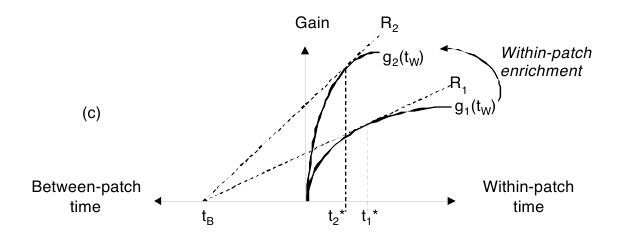
\includegraphics[width=0.8\textwidth]{enricment3.png}}
	\caption{(c) - Shows the changes generated by the adoption of within-patch enrichment strategies. The new gain function $g_2(t_w$) has a higher rate gain which  allows foragers that spend the same amount of time between patches $t_B$ will be able to reap more results in a shorter time.}
           \label{gain1}
\end{figure}

Figures (a), (b) and (c) are the graphical representation of the functions presented in the previous section according to Charnov's Marginal Value Theorem, they model the problem of allocation of time between in-patch vs. between-patch strategies. Here, between-patch search times $t_B$ , $t_{B1}$ and $t_{B2}$ generate different tangents to the $g(t_w)$ gain function which, in turn, determines the optimal rate of gain $R$. The outside of the curve on the x axis represents between-patch time while, the inside of it, represent within-patch time. To determine the optimal rate of gain $R*$ one draws the tangent line to the gain function $g(t_w)$ and passing through $t_B$ . The point of tangency will determine the "optimal allocation of within-patch foraging time $t*$".  

This means that, the more time is spent between-patch, the less a forager will find it beneficial to spend time exploiting a given patch, always depending on the gain function g(tw). In Figure 2, in fact, we see the effects of a between-patch enrichment like the one described previously (office re-disposition) which sets the optimal rate of gain in such a way that it will be more beneficial for the forager to spend more time within-patch to exploit it. Finally, in Figure 3 we can see the effect of within-patch enrichment (for instance, making information packages that yield better results). As we can see, within-patch enrichment, changes the gain function g(tw) determining higher gains per unit of time spent within-patch.

The objective of the experiment outlined in this proposal, is to be able to evaluate the strategies adopted by subjects in order to reach an optimal rate of gain and to analyse how they are able to choose between within/between-patch enrichment strategies to better their rate of gain per unit cost. 

\section{Searching Behaviour Games}

Throughout the years, several games to study searching behaviour have been developed. In this section we will explore the differences and similarities that these games have with Gold Digger. Even though these games involve a very different gameplay than Gold Digger, their objective has always been to test the user's ability in searching and information retrieval. In all of the previous games, in fact, the user is shown a particular web page and asked to retrieve it by typing queries in a search engine. In \textit{Page Hunt}, for example, the user is shown a difficult-to-retrieve page and is asked to input the appropriate query in a search engine in order to find it. \textit{Fu-Finder} instead, the user is asked to pick the most relevant link in the list returned by three different search engines. In both of these games, points are awarded either based on the number of pager found or on the number of pages as well as the rank at which those pages were retrieved. 

\textit{Page Fetch} and its second iteration \textit{Page Fetch 2} however, have a more complicated scoring system which introduces game dynamics that bring us closer to Gold Digger. In \textit{Page Fetch 2}, in fact, the user is encouraged to enter the shortest possible query in order to retrieve a particular page. This is done in order to discourage players from entering an obvious long query and instead be strategic, since the shortest query will yield the most points. In a similar way, in Gold Digger, the user that manages to dig least amount of layers while getting the greatest payoff is rewarded. 

 \textit{Page Fetch 2} also introduces a series of game features that are specifically aimed at enhancing the user experience and extending the amount of time users spend playing the game. These features include the awarding of badges and the ranking of players in leaderboards, so that they can compare their performance against other players and strive to be the best. Gold Digger also incorporates these features (see ~\ref{subsec:achievements}) and tries to expand them further in the direction of an even more enhanced gaming experience. In addition to this, \textit{Page Fetch 2}, allows the user to choose between different categories of similarly themed web pages. In the same way, In Gold Digger offers the user a series of different locations in which to play.

%%%%%%%%%%%%%%%%%%%%%%%%%%%%%%%%%%%%%%%%%%%%%%%%%%%%%%%%%%%%%%%%%%%
\chapter{Design}\label{design}

The design of Gold Digger went through different iterations through the course of its development (see 4.2 Heuristic Evaluation), however some design choices were made in order to keep the user experience consistent throughout the website and enhance clarity and ease of use.

\textbf{Separation between "game pages" and "site pages"}

Because Gold Digger is both a website and a game, it seemed appropriate to somehow separate the "game environment" from the more "site-like" features and pages, while still maintaining a certain degree of coherence between them. "Game pages" are the ones immediately relevant to the game in itself, the ones that the user will most likely enter while playing Gold Digger. These are: \textbf{the Game/Mine page, the General Shop page, the Home Page} and \textbf{the World Map Page}. The other pages are said to be "site pages" and they include pages like the About page and the Leaderboards, which a user is not very likely to access while in the middle of a play through. Furthermore "game pages" all require the user to be logged in to be accessed while the "site pages" do not. 
\\*
Notwithstanding this distinction, the user experience is not disjointed thanks to prominent recurring elements such as the nav bar on the top of the page and the landscape headline showing the name of each page.

\section{Site Map}

\begin{figure} [!ht] 
	\centering
           \makebox[\textwidth][c]{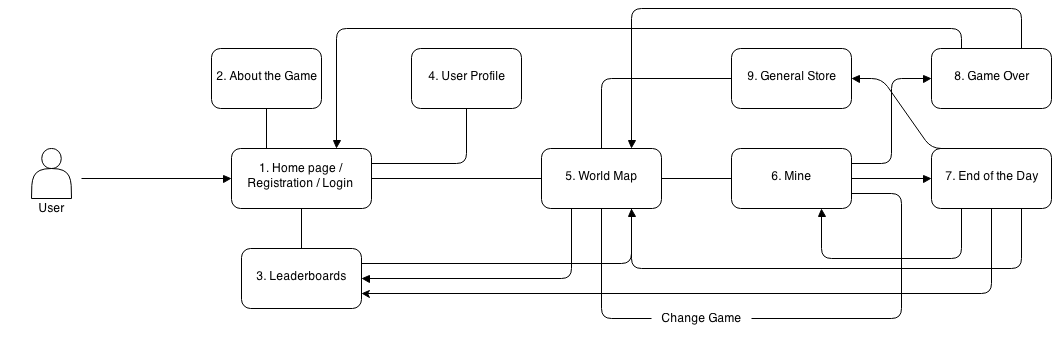
\includegraphics[width=1\textwidth]{sitemap.png}}
	\caption{Gold Digger nav bar}
           \label{navbar}
\end{figure}

Navigation through the website is aided by a navbar located at the top of every page (with the exception of the 'game over' and 'end of the day'
pages). 
\begin{figure} [h] 
	\centering
           \makebox[\textwidth][c]{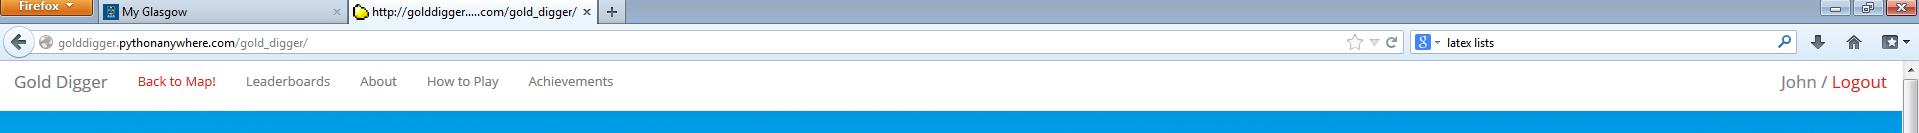
\includegraphics[width=1\textwidth]{nav.png}}
	\caption{Gold Digger nav bar}
           \label{navbar}
\end{figure}

From the navbar the user will be able to reach the following pages:

\begin{itemize}
  	\item The main page (by clicking on 'Gold Digger')
  	\item The World Map page (if signed in)
	\item The Leadeboards
	\item The About page
	\item The 'How to Play' / Tutorial page
	\item The 'Achievements' page
  	\item The User Profile page (if signed in)
\end{itemize} 

finally, the user will also be able to logout at any moment by using the 'Logout' button on the top right. However, if the user is currently in one of the mines,
clicking on one of these links will result on a warning message being displayed that will alert users that the gold gathered during the day will be lost if they leave
the mine before exhausting the time at their disposal and reaching the end of the day. 

\subsection{Home, Registreation and Login}


\begin{figure} [h] 
	\centering
           \makebox[\textwidth][c]{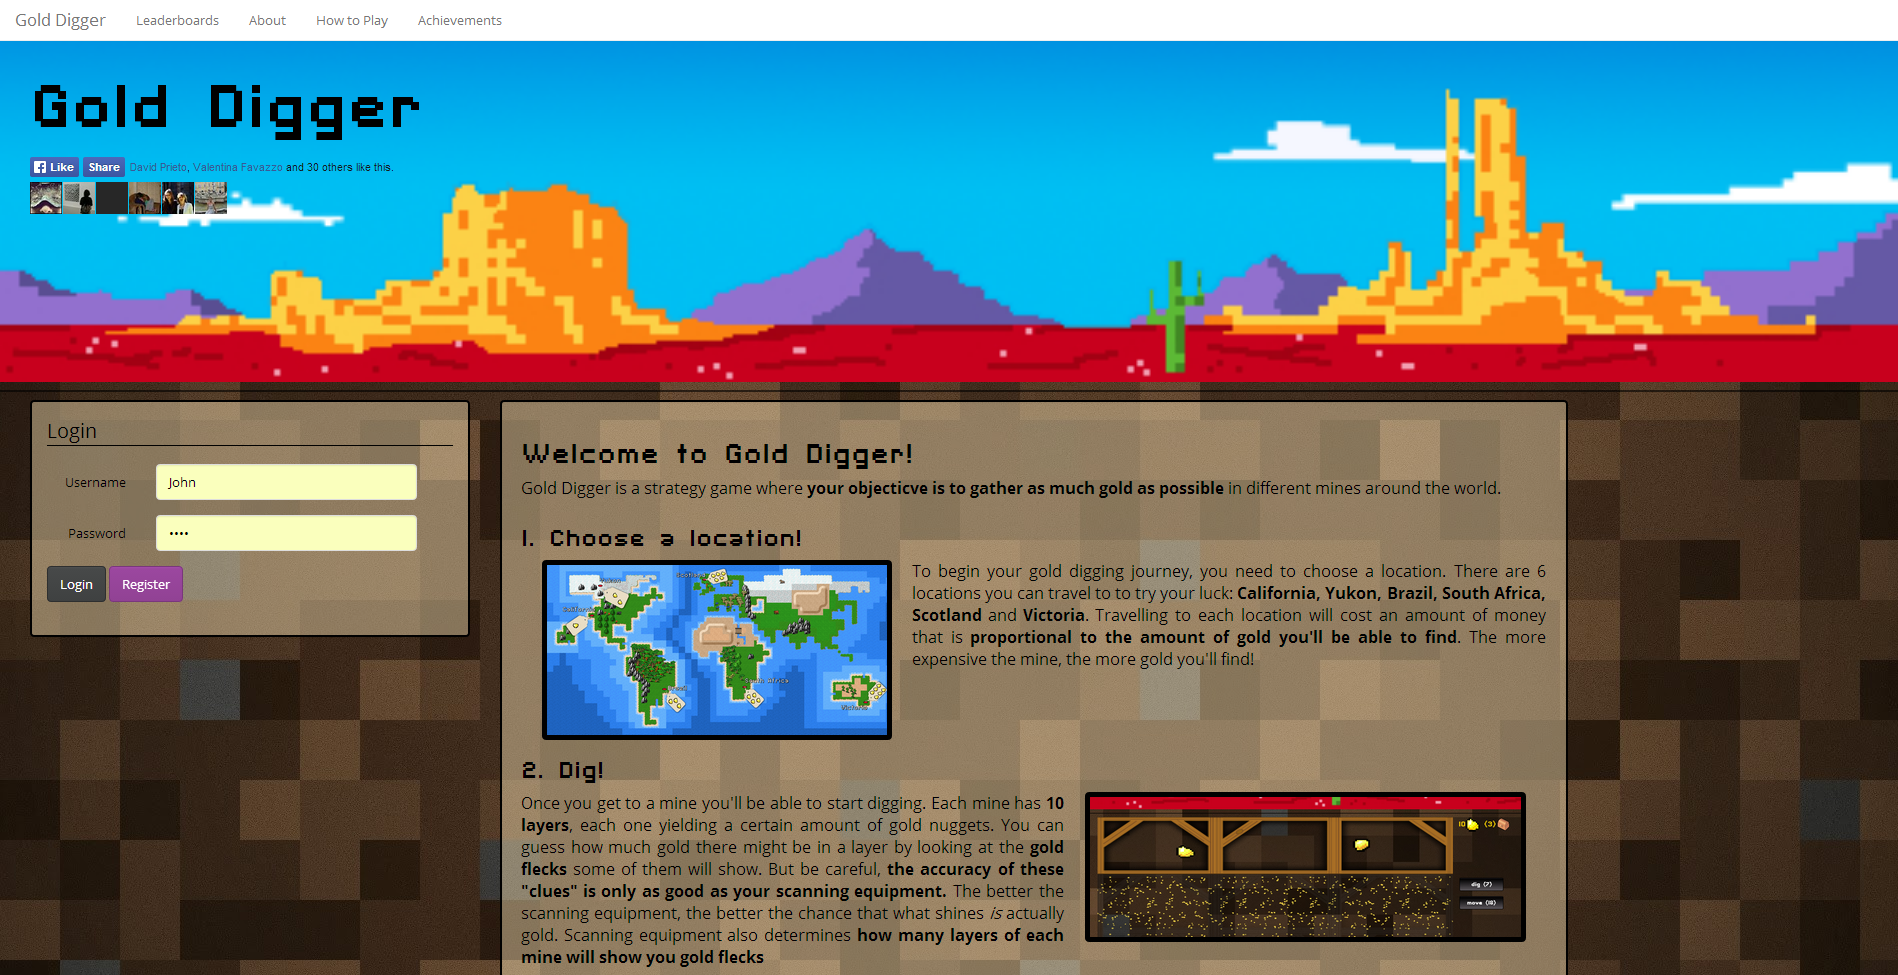
\includegraphics[width=1.2\textwidth]{homescreen.png}}
	\caption{Home Page}
           \label{homepage}
\end{figure}

On the landing page (homepage) users will be presented with a short \textbf {five-point explanation} of the game to quickly explain the mechancs of the game so that
users could start playing as soon as poosible. To so this, they will have to login through the form on the left or register by clicking on the 'Register' button. 
\begin{figwindow}%
[0, r, 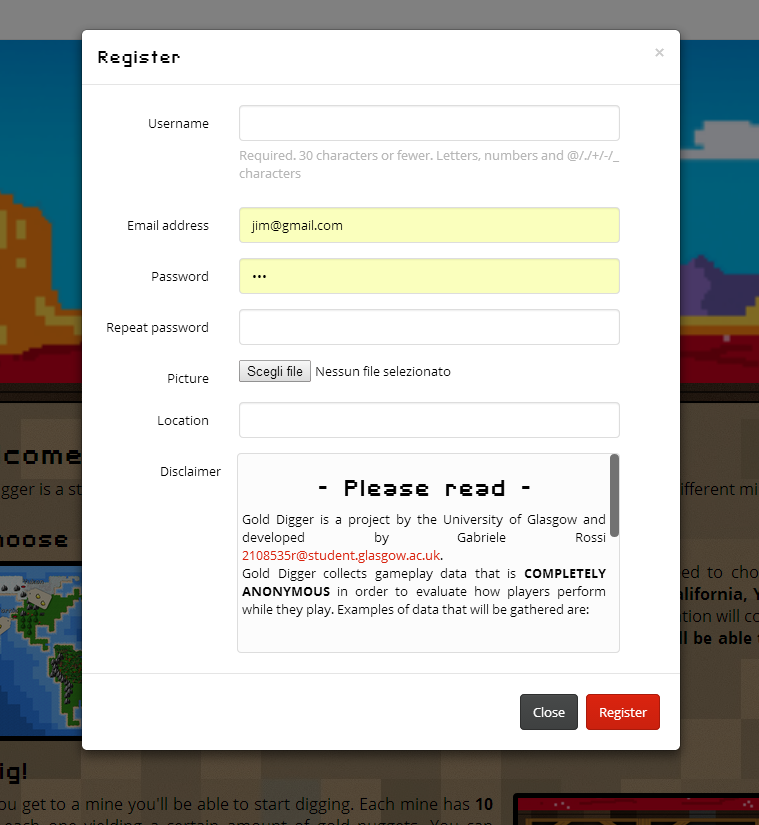
\includegraphics[width=.5\textwidth]{register.png},%
{ Registration modal}]
Clicking on the \textbf{ 'Register'} button will trigger a modal asking users to create a new username and password, as well as optionally entering their location and user
picture. Finally, the modal displays a disclaimer in order to both make sure that the users are aware of the limitations of accessing the website and its purpose. 
Users who wish to have more information about Gold Digger are redirected to the 'About' page or offered a link to directly write an email to the developer.
\\
Finally if a user enters wrong details or forgets to fill in a required field, (both for registration and login) an appropriate error message is clearly displayed for the user to see and try again. 
At present there is no limit to the number of attempts a user can make at logging in or registering.

\end{figwindow}

\subsection{World Map}

\begin{figure} [h] 
	\centering
           \makebox[\textwidth][c]{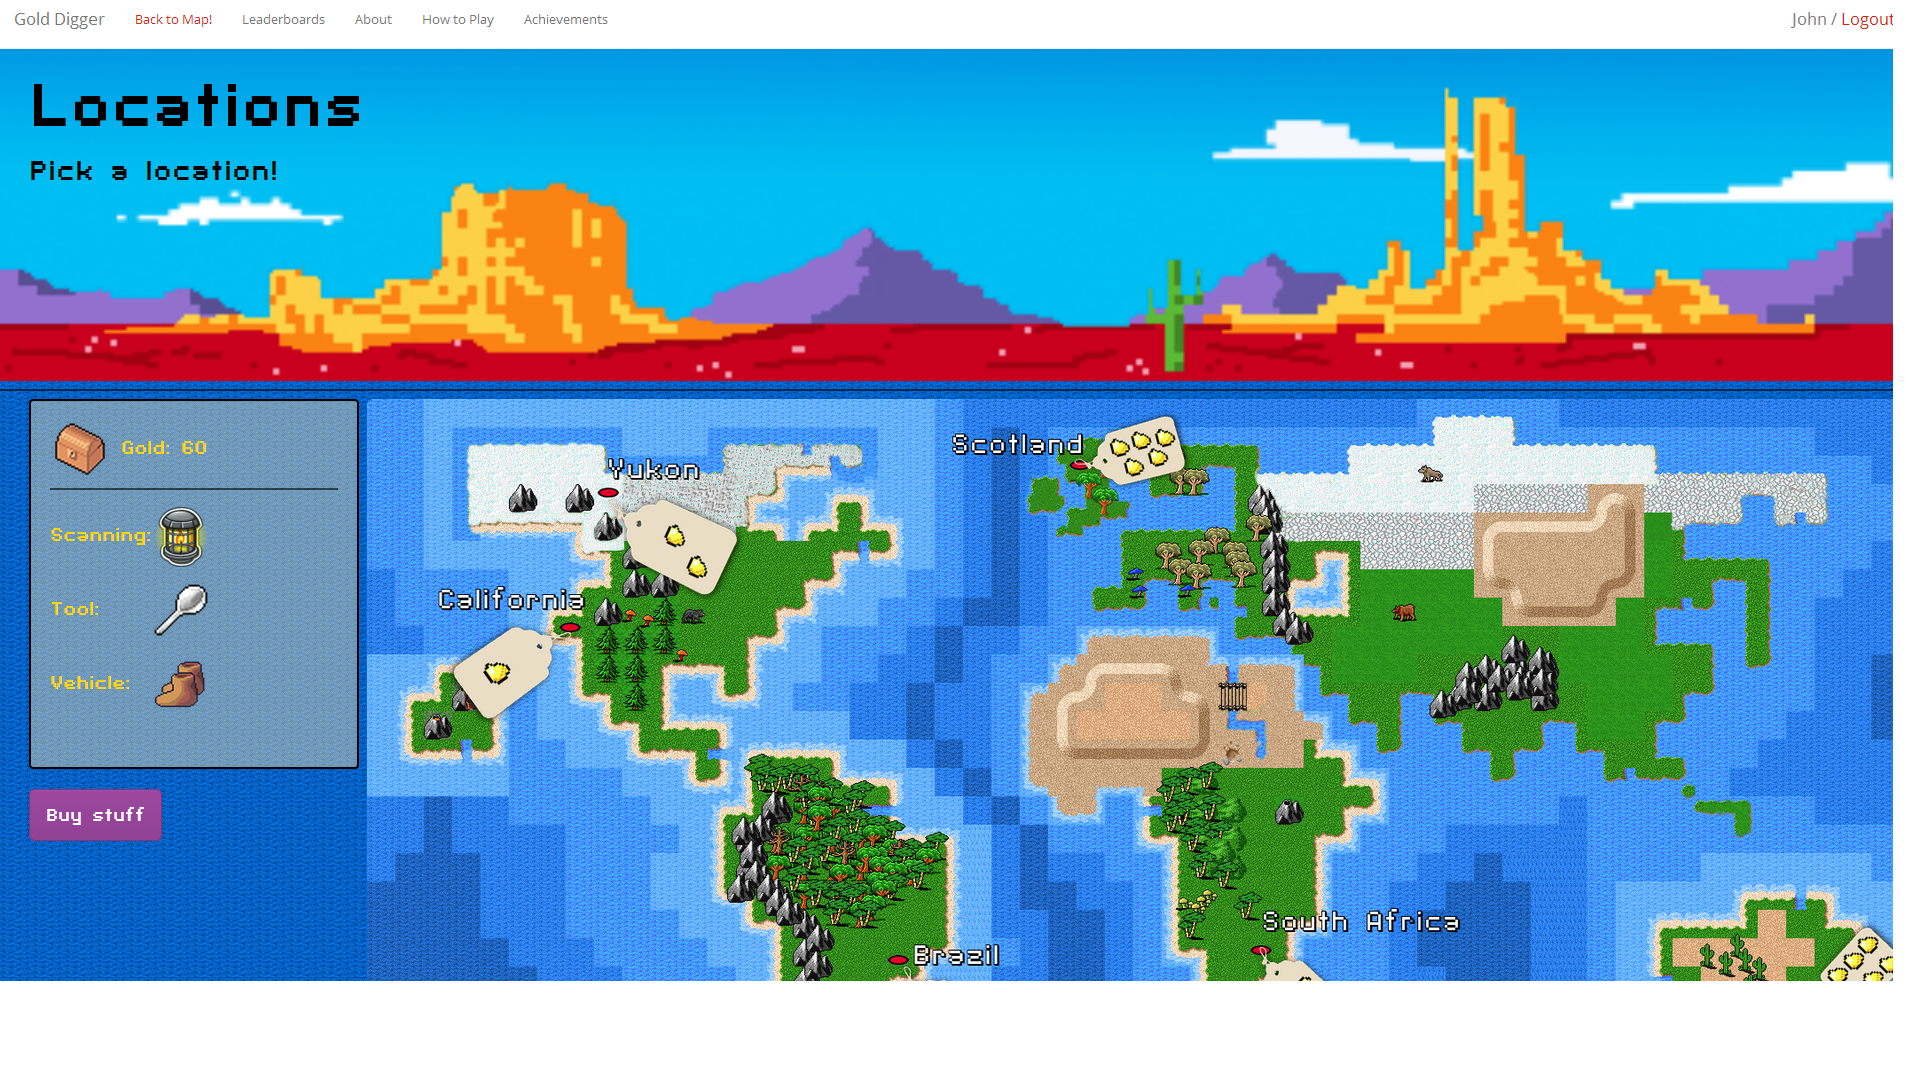
\includegraphics[width=1.2\textwidth]{worldmap.png}}
	\caption{World Map}
           \label{worldmap}
\end{figure}

Once users have registerd or have been logged in, they are automatically redirected to the world map so that they can start playing immediately. 
On the left of the page, users can see the euqipment and the amount of gold they have at the moment. The side item panel appears on the left column of the page, once the user has logged in. The panel shows the items that users have equipped, together with the total amount of gold in their possession. By hovering over each one of the items a tooltip will appear, showing the essential stats of each item. The presence of the side item panel has the function of both confirming the users that they are logged in and  reminding them that their game session has started  contributing to the uniformity of the user experience.
\begin{figwindow}%
[0, l, 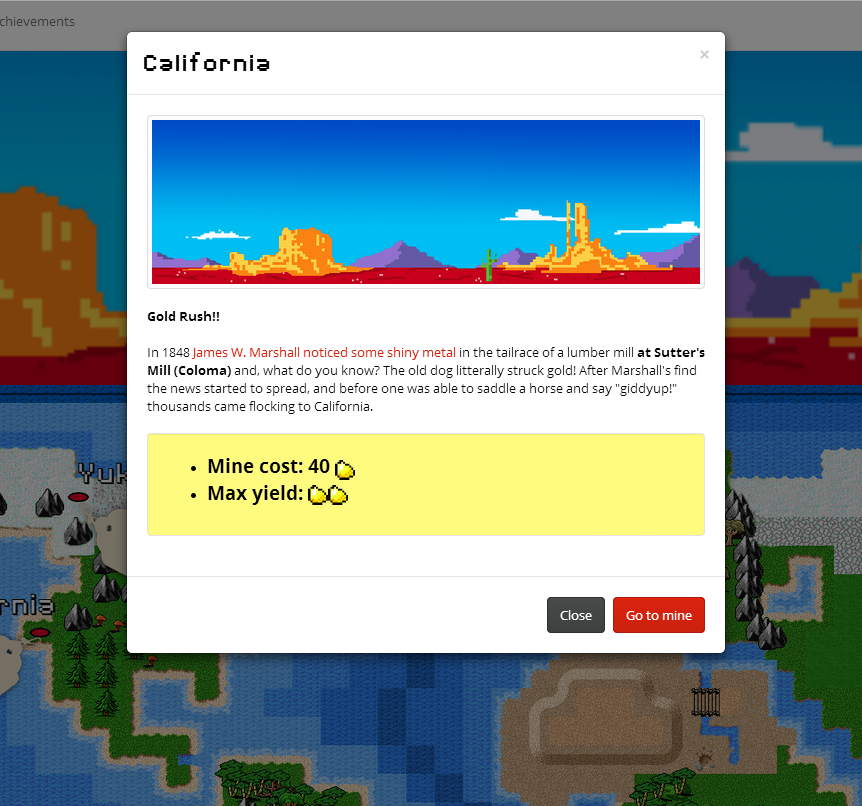
\includegraphics[width=.4\textwidth]{cali.png},%
{ California modal}]
 On the right hand side of the page users can access any of six locations: \textbf{California, Yukon, Brazil, South Africa, Scotland} and \textbf{Victoria}. 
Clicking on any of the locations will trigger a modal that displaying the scenery of the particular mine, some information about the gold digging history in that region (with links to Wikipedia articles), the cost of the mine and the amount of gold the user can expect to find. Starting from California and ending with Victoria, each mine is more expensive than the previous one 
but it also have a potentially higher gold yield. It is up to the player to enter the right mine at the right time.
\end{figwindow}

\subsection{Game Screen}
\begin{figure}[h] 
	\centering
           \makebox[\textwidth][c]{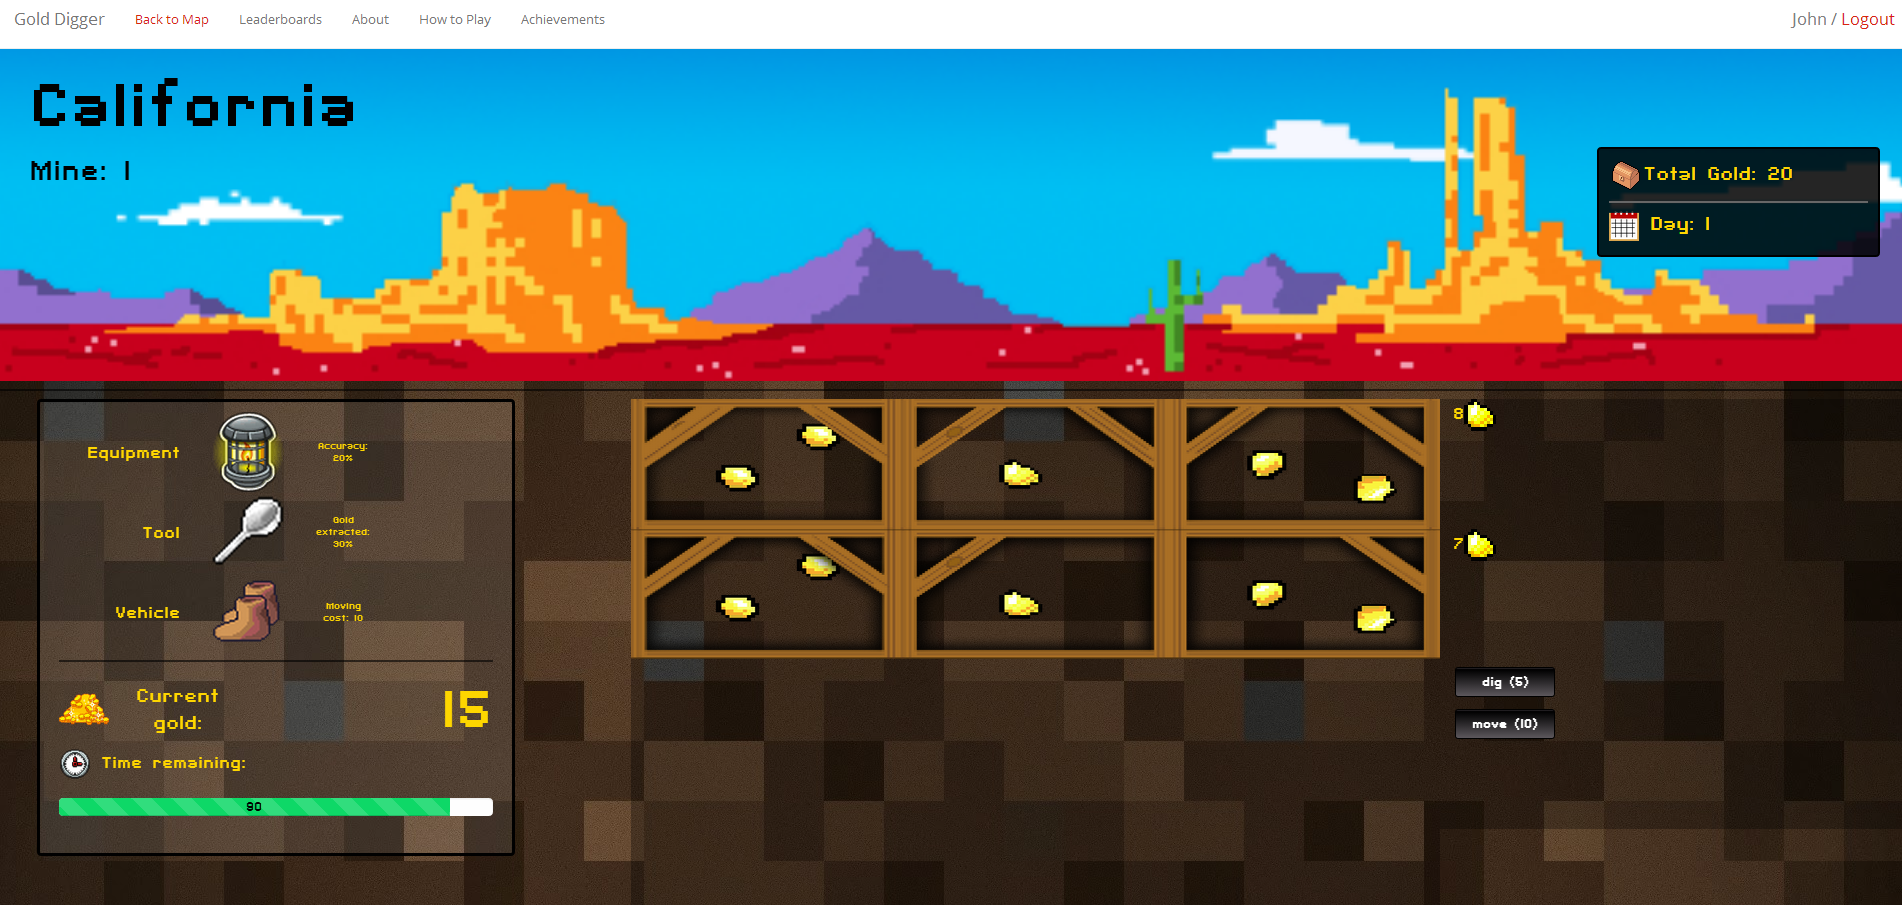
\includegraphics[width=1.2\textwidth]{mine.png}}
	\caption{Mine}
           \label{mine}
\end{figure}

Once the users enter a mine, the appropriate amount of gold is removed from the total and they can start digging. Each mine presents a similar structure, except for the landscape and the
amount of gold that can be found in each layer. On the top of the page we can see the landscape picture and the name of the location, as well as the number of mines that the user has dug into during the present day. As previously noted, on the left, we can find the equipment panel, in the middle we have the mine shaft and on the right have the \textbf {'Dig'} and \textbf{'Move'} as well as the yield of each layer that has been already dug. The left side panel contains here some more information than it does in the other pages where it appears:
\begin{itemize}
  	\item \textbf{Current gold}: the amount of gold gathered during the present day.
  	\item \textbf{Time remaining}: the amount of time (in units of time) remaining before the end of the day.
\end{itemize} 
Furthermore, because the left side panel's position is fixed, it will follow users as they get deeper and deeper in the mine, allowing them to always keep an eye on the game state without having to go back to the top of the page to check how many units of time they have left before the end of the day. Because the 'Current gold' is summed to the 'Total Gold' only at the end of the day, the total amount of gold, together with the number of days users have been digging without encountering a game over, is displayed in a small box on the top right of the page.
 The options available to the user and an example of gameplay are detailed in section 3.2.

\subsection{General Store}

\begin{figure} [h] 
	\centering
           \makebox[\textwidth][c]{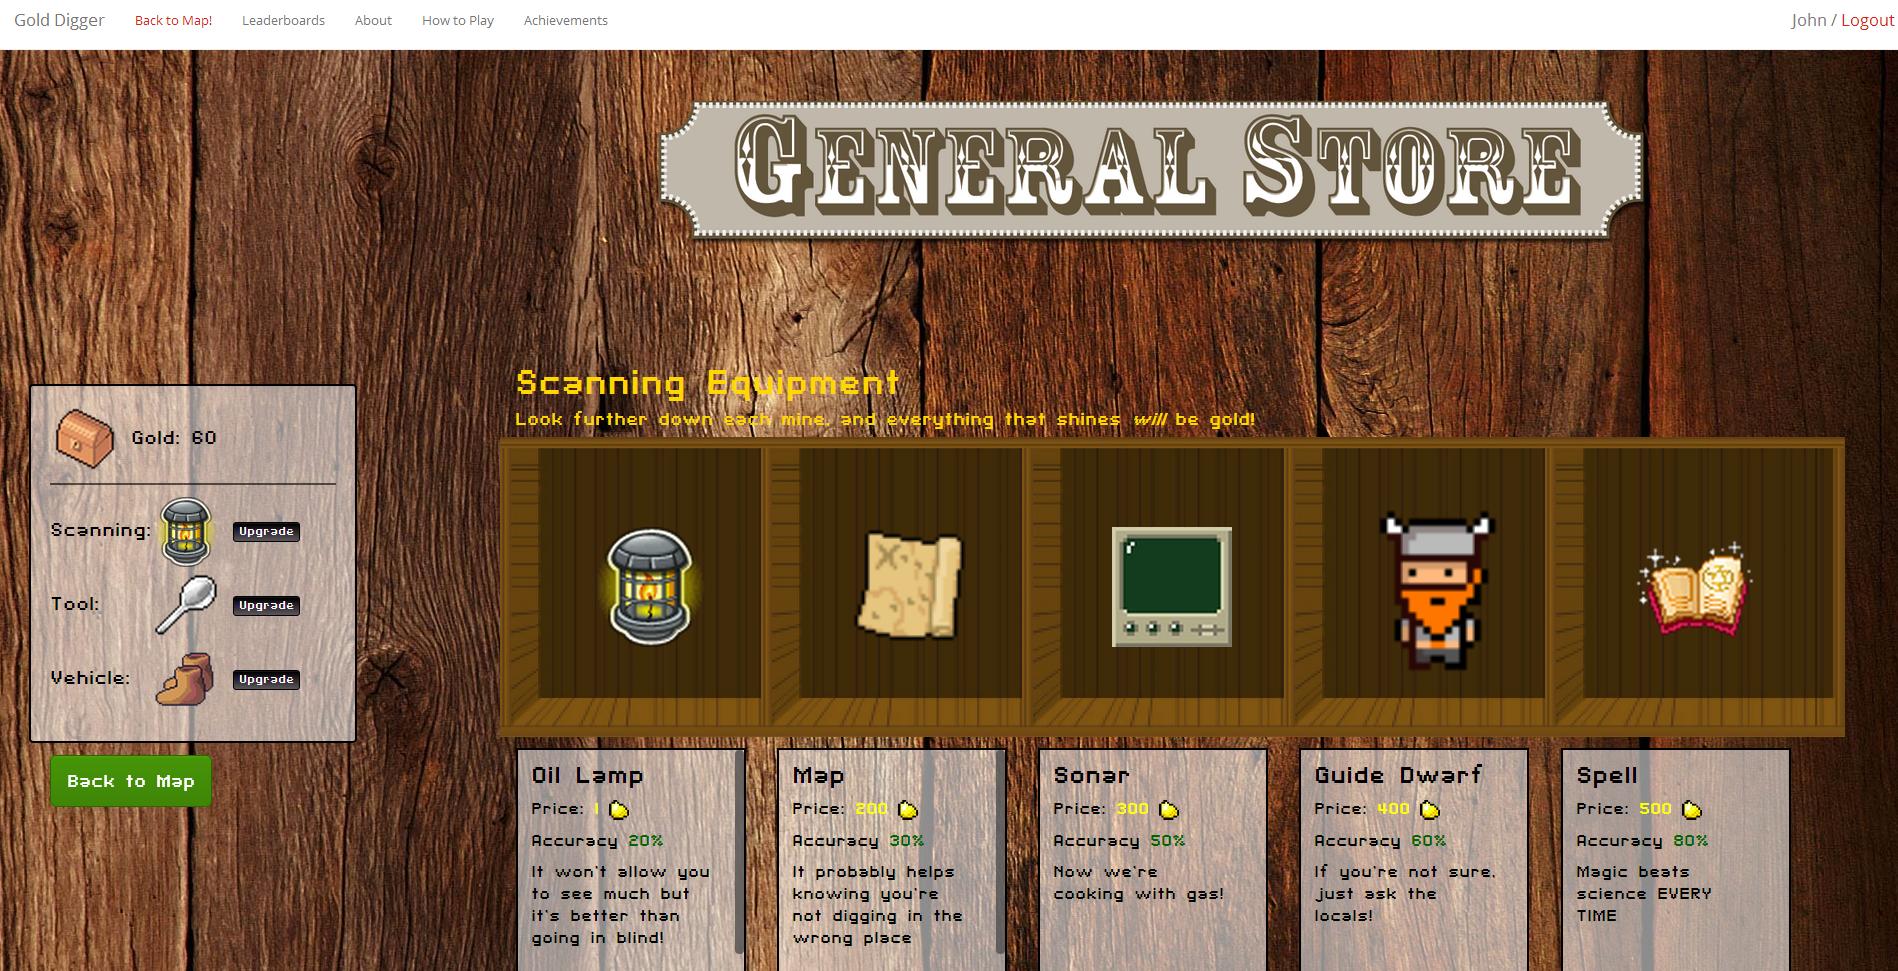
\includegraphics[width=1.2\textwidth]{generalstore.png}}
	\caption{General Store}
           \label{fig: generalstore}
\end{figure}

At the end of each day (by clicking on \textbf{'shop'}), or from the world map screen (by clicking on \textbf{'Buy stuff'}), users can access the \textbf{General Store} (see fig. \ref{fig: generalstore}). From here they are able to browse and purchase new items to help them in their digging. There are three groups of objects that the user can choose from \textbf{Scanning Equipment, Digging Equipment} and \textbf{Vehicles}. Each of these groups contains five different items with different cost and stats. Users are able to see the image associated with each item as well as its cost,  stats and a short description in the small tex box underneath. If users decide to upgrade one of their item groups (Scanning, Digging or Vehicle) they can do so by clicking on the \textbf{'Upgrade'} button. At this point they will be presented with a small modal that reviews the item's stats, together with its picture, asking the user to confirm the purchase. If the users don't have enough gold to make the purchase, or if the purchase would cause them to not have enough money to enter the cheapest mine, an appropriate alert message is displayed, explaining why the purchase is not possible.

The choice to allow users to \emph{upgrade} rather that \emph{buy} items has been made because each of the items is better than the previous one in every respect and thus there is no reason why a user would chose to equip an item that they previously purchased, since this would not bring any advantage at all. For instance, with digging tools, their cost, dig cost (the amount the user has to pay in time units to dig once) and extraction power (the percentage of gold that the user will be able to extract given a certain yield), are all increased from the least, to the most expensive. However, it would be easy to add items that have different combinations of these parameters and add, for example, a digging tool that, at a higher cost per dig also returns a higher percentage of gold.
Finally, upon purchase, the new item is immediately added to the left side panel and the appropriate amount of money removed from the user's total through an AJAX call.

 \subsection{Leaderboards}

\begin{figure} [h] 
	\centering
           \makebox[\textwidth][c]{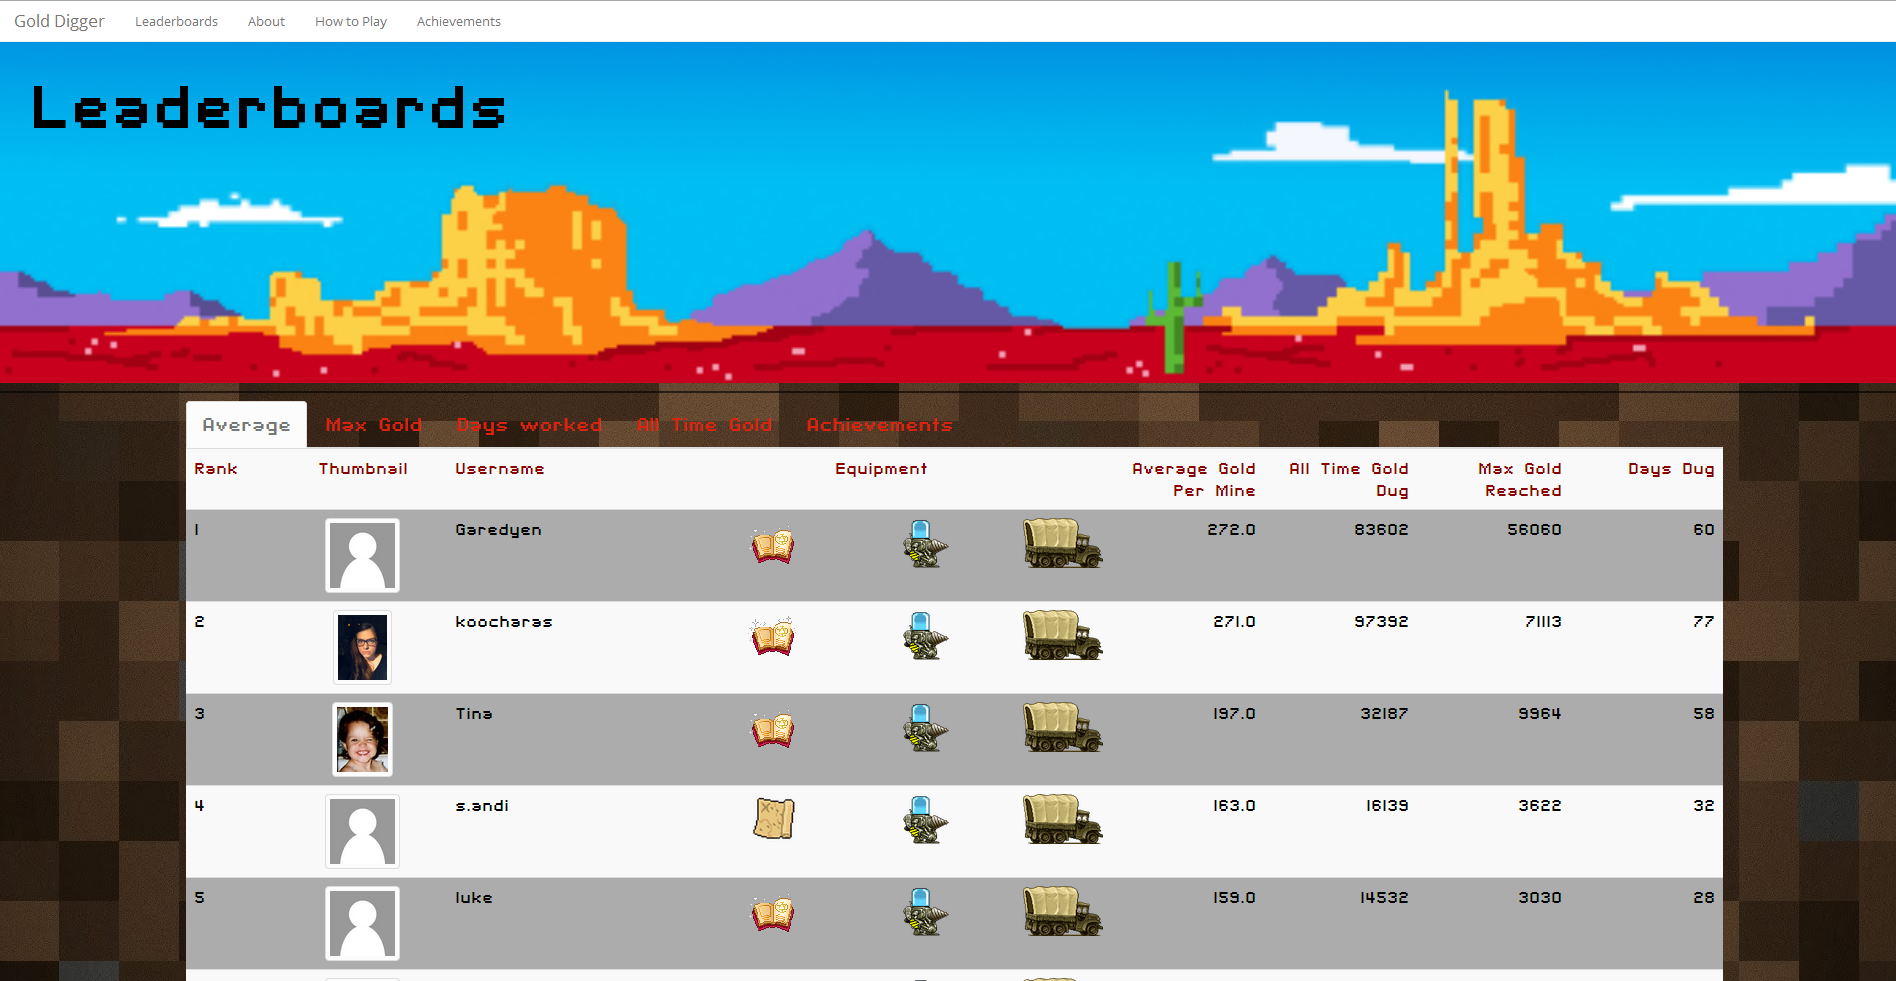
\includegraphics[width=1.2\textwidth]{leaderboards.png}}
	\caption{Leaderboards}
           \label{fig: leaderboards}
\end{figure}

On the \textbf{Leaderboards} (see fig. \ref{fig: leaderboards}) page, users are able to check their performance and compare it to the other players'. There are four parameters by which users can be ranked, plus an achievements board that has no specific ranking criteria: 

\begin{itemize}
  	\item \textbf{Average}: the total amount of gold ever dug by the player divided by the total amount of mines that were dug into.
  	\item \textbf{Max Gold}: the maximum amount of Gold ever dug (the maximum amount of gold ever reached)
	\item \textbf{Days Worked}: the total amount of days of digging completed by the player (not zeroed on game over)
	\item \textbf{All Time Gold}: the cumulative total amount of gold dug by the player  (not zeroed on game over)
	\item \textbf{Achievements}: shows the achievements gained by each player in no particular order (achievements are not ranked)
\end{itemize} 

Each row of the the tables (excluding the 'Achievement' table) diplays the following parameters: Rank, Thumbnail, Username, Equipment (showing the image for each of the three item groups), Average Gold per Mine, All Time Gold Dug, Max Gold Reached, Days Dug.

\subsection{Tutorial}

\begin{figure} [h] 
	\centering
           \makebox[\textwidth][c]{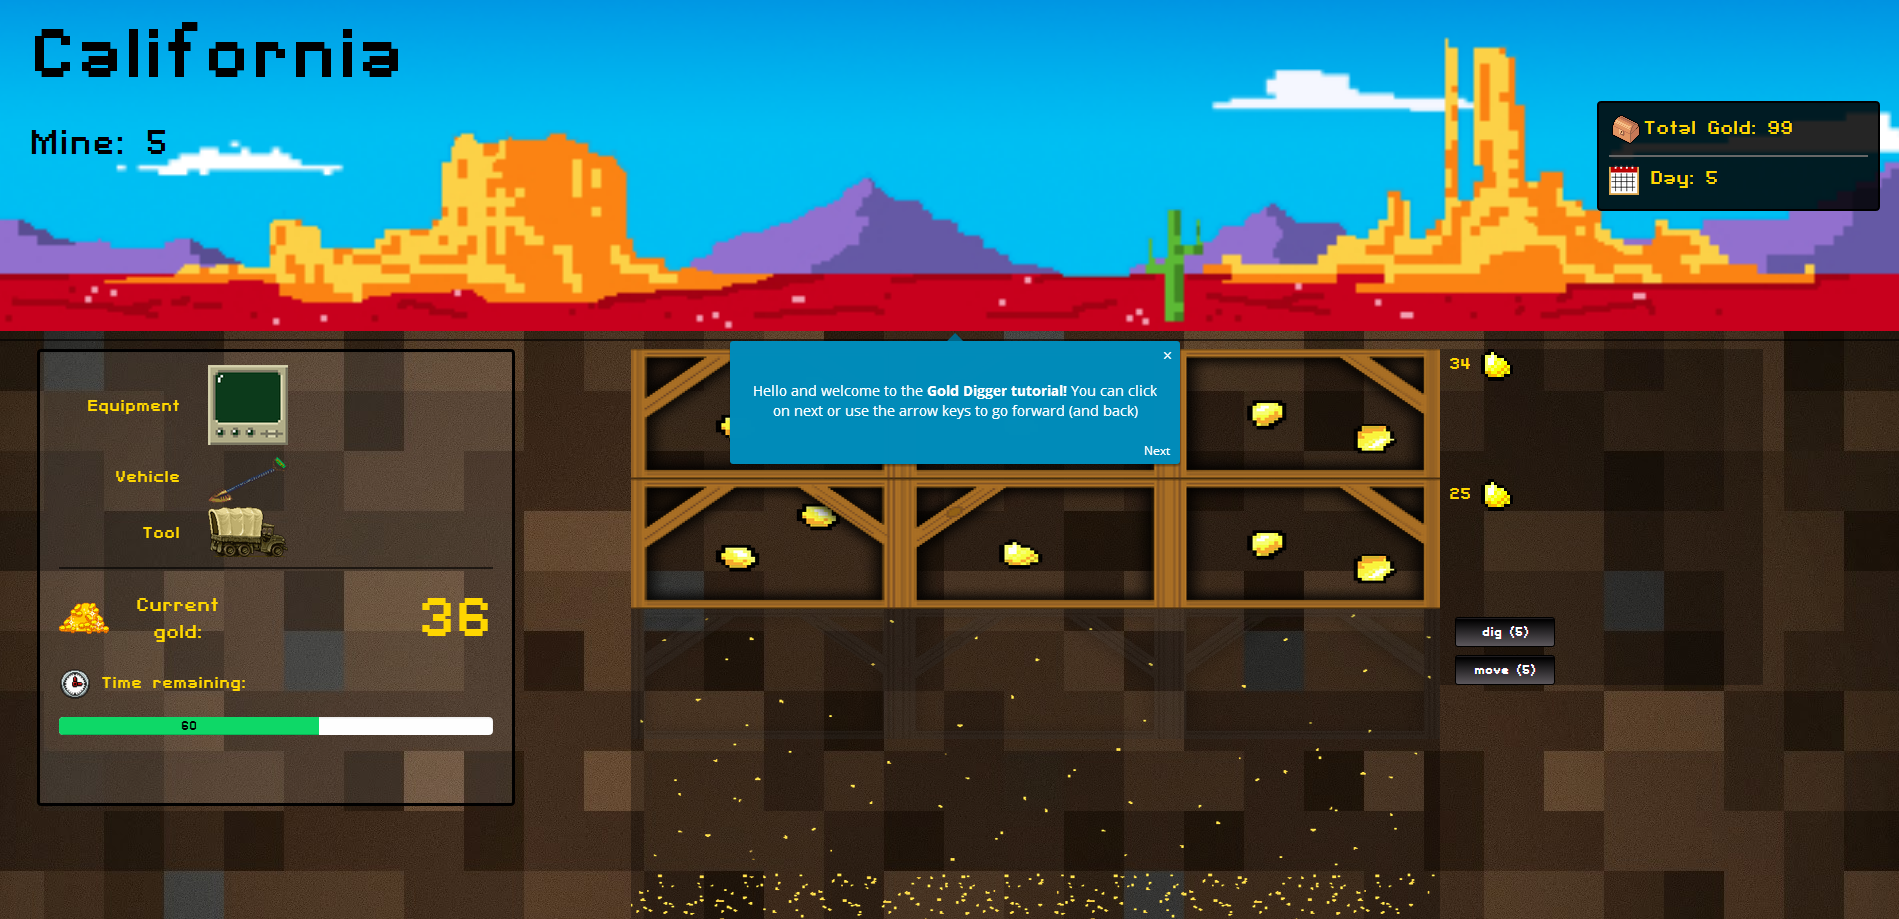
\includegraphics[width=1.2\textwidth]{tutorial.png}}
	\caption{Tutorial}
           \label{fig: tutorial}
\end{figure}

Because it is important for users to have a clear idea of the way the game works, all effort has been made to employ a visual approach that would be quick and easy to understand. To this end, upon entering, the \textbf{'How to Play'} page, a tour of the main game features is automatically launched. The javascript library \textbf{Trip.js} (see 4.4.6) highlights and points at the different parts of the game screen in order to get a quick visual explanation of the main game mechanics. Each of the labels has 'Next', and 'Previous' link, in order to let users go back to a previous point or skip explanations they already viewed.

\subsection{Achievements}
\label{subsec:achievements}
\begin{figure} [!hb] 
	\centering
           \makebox[\textwidth][c]{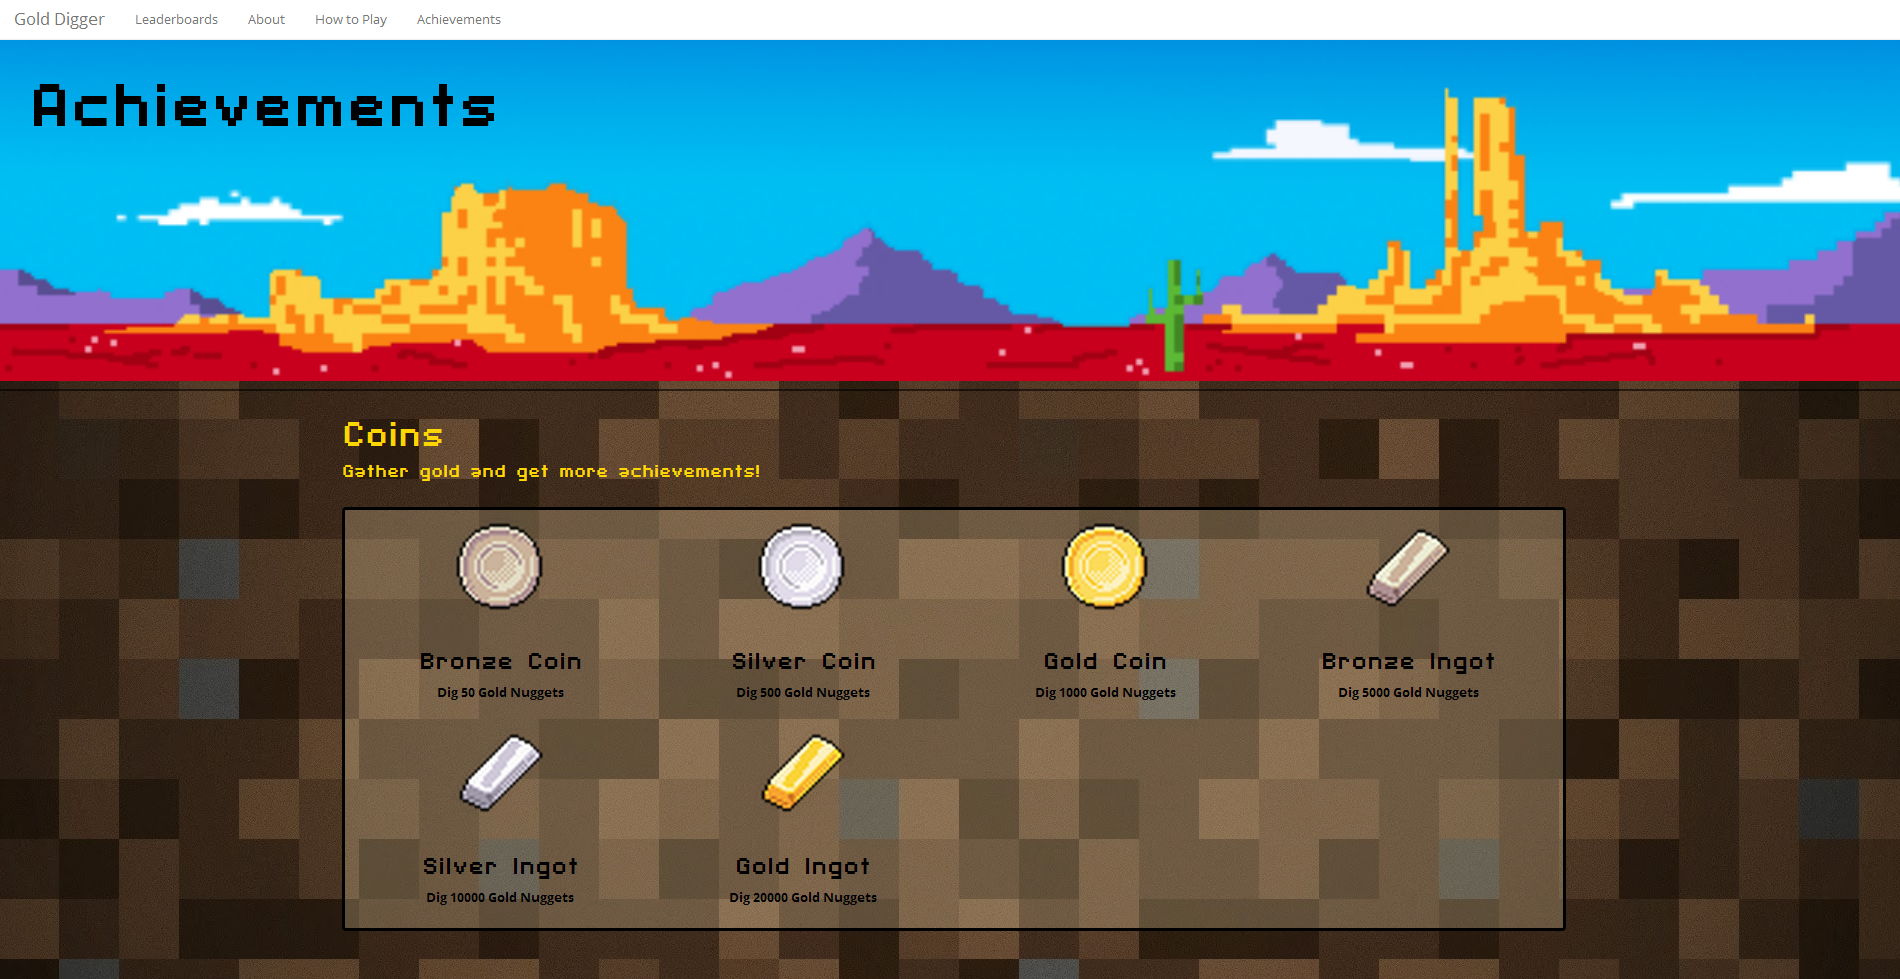
\includegraphics[width=1.2\textwidth]{achievements.png}}
	\caption{Achievements display}
           \label{fig: achievements}
\end{figure}

The \textbf{'Achievements'} page dispays all the achievemts badges together with their name, the condition that triggers them and their image. This page is needed in order for the users to be able to check which achievements they can aim for while playing. Two additional achievements (fig. \ref{fig: specialachievements}) are not displayed here and are given only under special conditions:

\begin{figure}[!h]
        \centering
        \begin{subfigure} [!h] {0.4\textwidth}
                \centering
                
\includegraphics [width=0.4\textwidth] {awesome.png}
                \caption{You helped testing!}
                \label{}
        \end{subfigure}
        \space
        \space
        \begin{subfigure} [!h] {0.4\textwidth}
                \centering
                
\includegraphics [width=0.4\textwidth] {banana.png}
                \caption{You found the Easter Egg!}
                \label{}
        \end{subfigure}
        \caption{Special Achievements}
        \label{fig: specialachievements}
\end{figure}

\begin{itemize}
  	\item \textbf{Awesomeness}: given to the people who tested the "beta" version of the site.
  	\item \textbf{Banana}: given to people who managed to find the game's Easter Egg
\end{itemize} 

Achievements ans special achievements have been incorporated in order to both add an extra game feature to Gold Digger which wouldn't change the game mechanics too much an to give players an incentive to keep playing, especially since there is no particular "winning condition", fulfilled which a player has completed the game.  

\subsection{About Page}

In this page, users are able to find  the developer and supervisor's contact details as well as reading about the reasons behind the creation of Gold Digger and acknowledgements of the authors of some of the material used in the site.


\section{Walkthrough}

\begin{figure}[!h]
        \centering
        \begin{subfigure} [h] {0.6\textwidth}
                \centering
                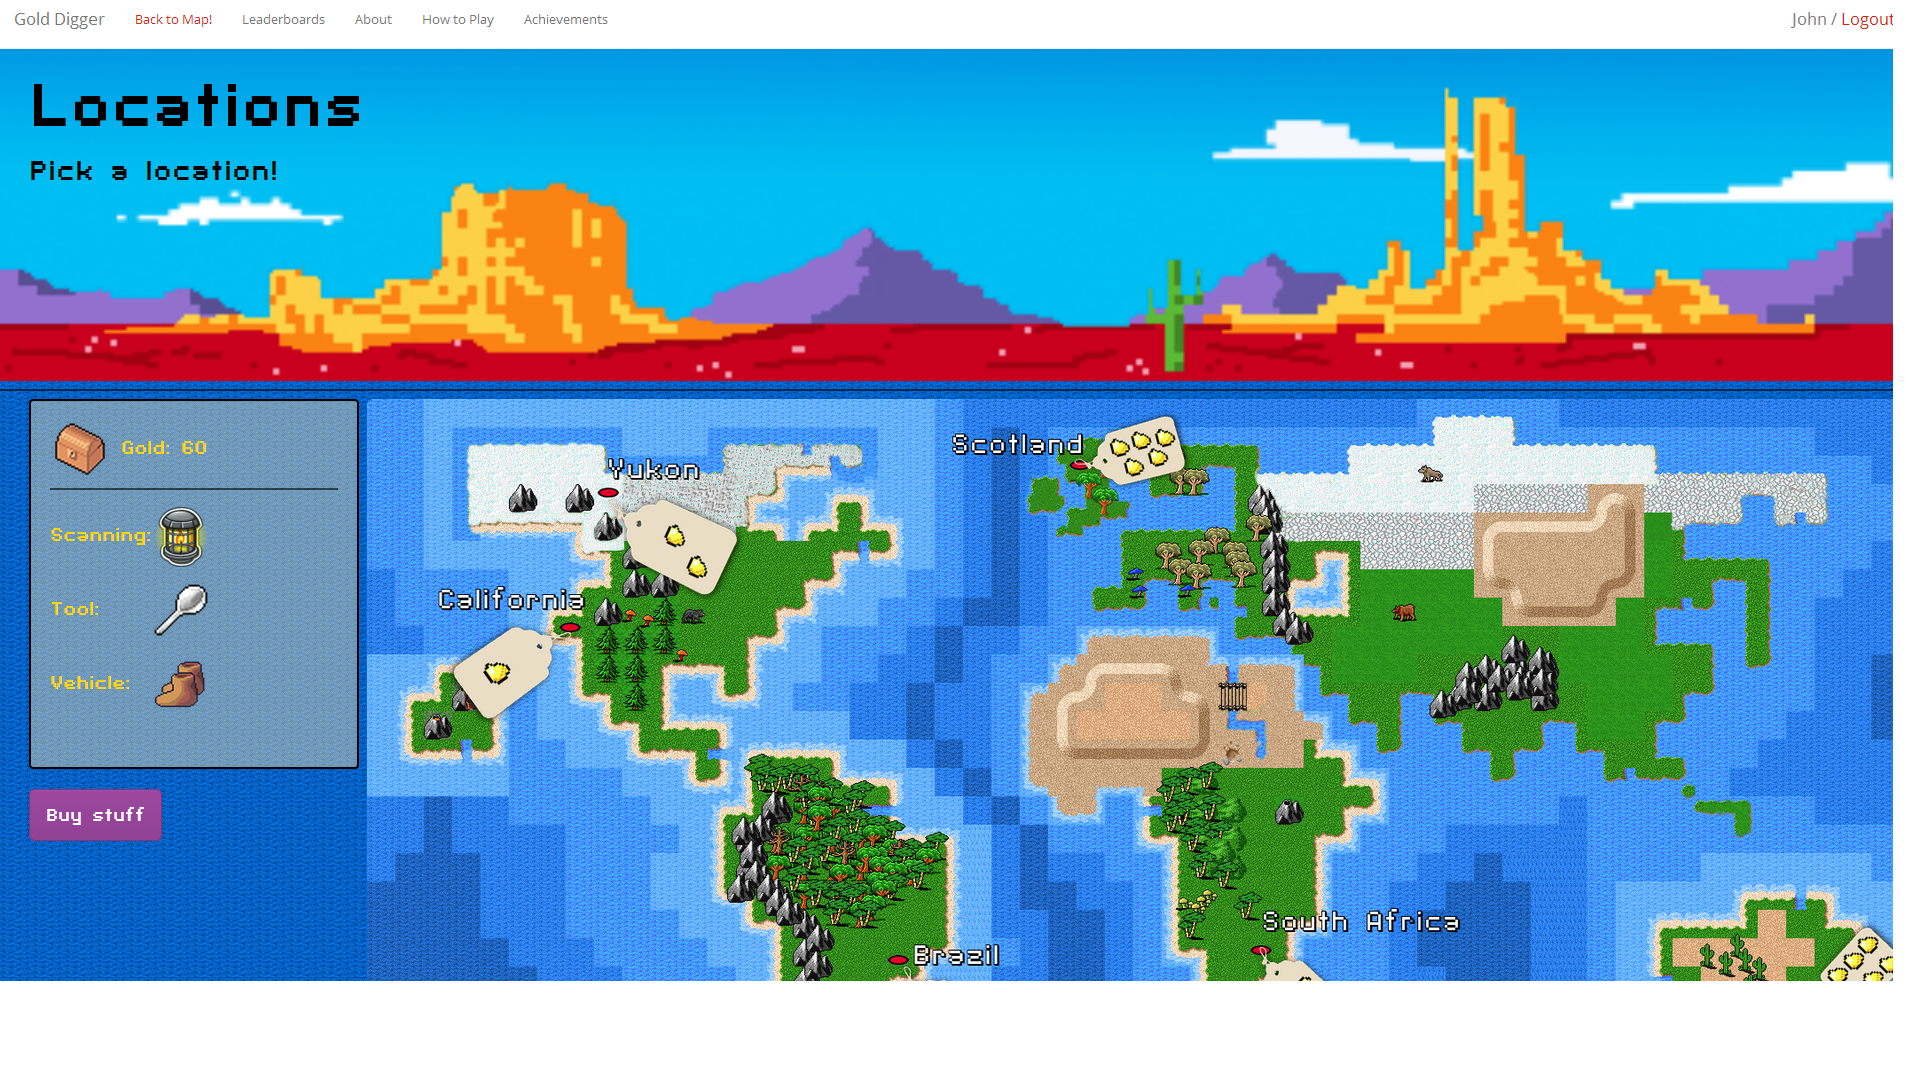
\includegraphics [width=1\textwidth] {worldmap.png}
        \end{subfigure}
        \space
        \space
        \begin{subfigure} [h] {0.3\textwidth}
                \centering
                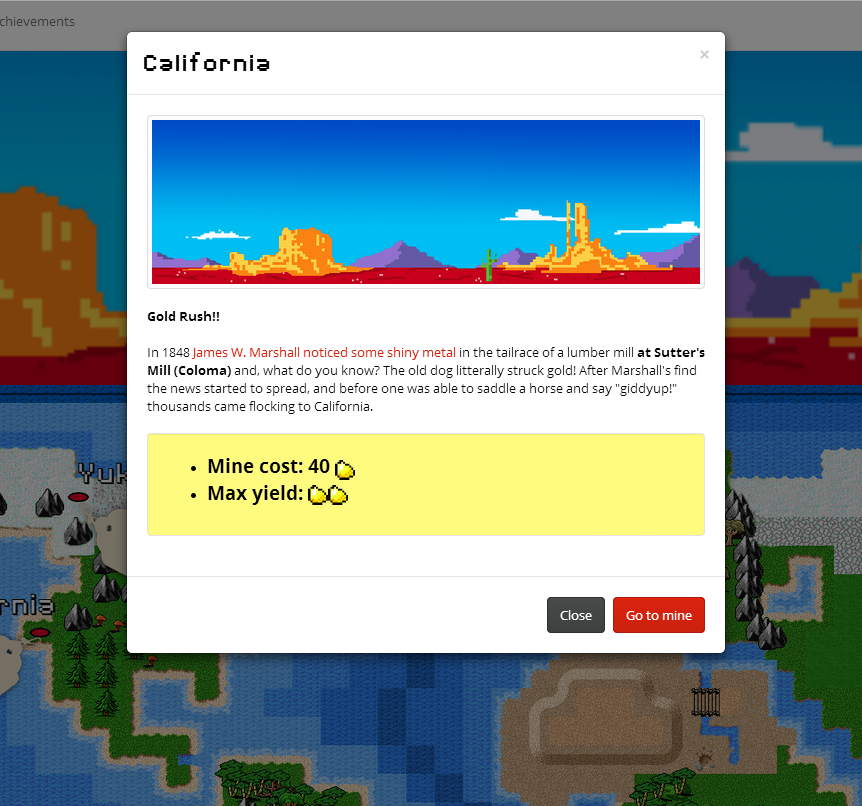
\includegraphics [width=1\textwidth] {cali.png}
        \end{subfigure}
\end{figure}

(1) Jill, the user, has just logged in (or registered) and has been redirected to the World Map. Her starting Equipment and Gold are as follows:
\begin{itemize}
	\item \textbf{Gold}: 100
  	\item \textbf{Scanning Tool}:  Oil Lamp (accuracy: 20\%, visibility: 2)
  	\item \textbf{Digging Tool}: Spoon (dig cost: 5, gold extracted 30\%)
	\item \textbf{Vehicle}: Boots (move cost: 10)
\end{itemize} 

On the map, Jill clicks on California and a modal appears, from which she can see see that, although the mine doesn't yield much gold, it is relatively cheap to access it (she only needs to pay 40 gold nuggets to enter it).

(2) After clicking on 'Go to Mine', 40 gold nuggets are removed from Jill's total amount of gold and she is presented with a mine where no layer has been dug(fig~\ref{fig:two}). On the top left hand side Jill can see the name of the location she is in and the number of the mine (now 1) whereas on the right hand side she can check her total amount of gold (now 60) and the number of days she has been digging. Thanks to her Oil Lamp she can see specks of gold in the first two layers but, because the lamp only has a 20\% accuracy, it is possible that the amount of flecks that can be seen is deceiving. 

\begin{itemize}
	\item \textbf{Current gold}: 0
  	\item \textbf{Time remainingl}: 100
  	\item \textbf{Mine}: 1
	\item \textbf{Day}: 1
\end{itemize} 

\begin{figure}[!ht]
        \centering
        \begin{subfigure} [h] {0.45\textwidth}
                \centering
                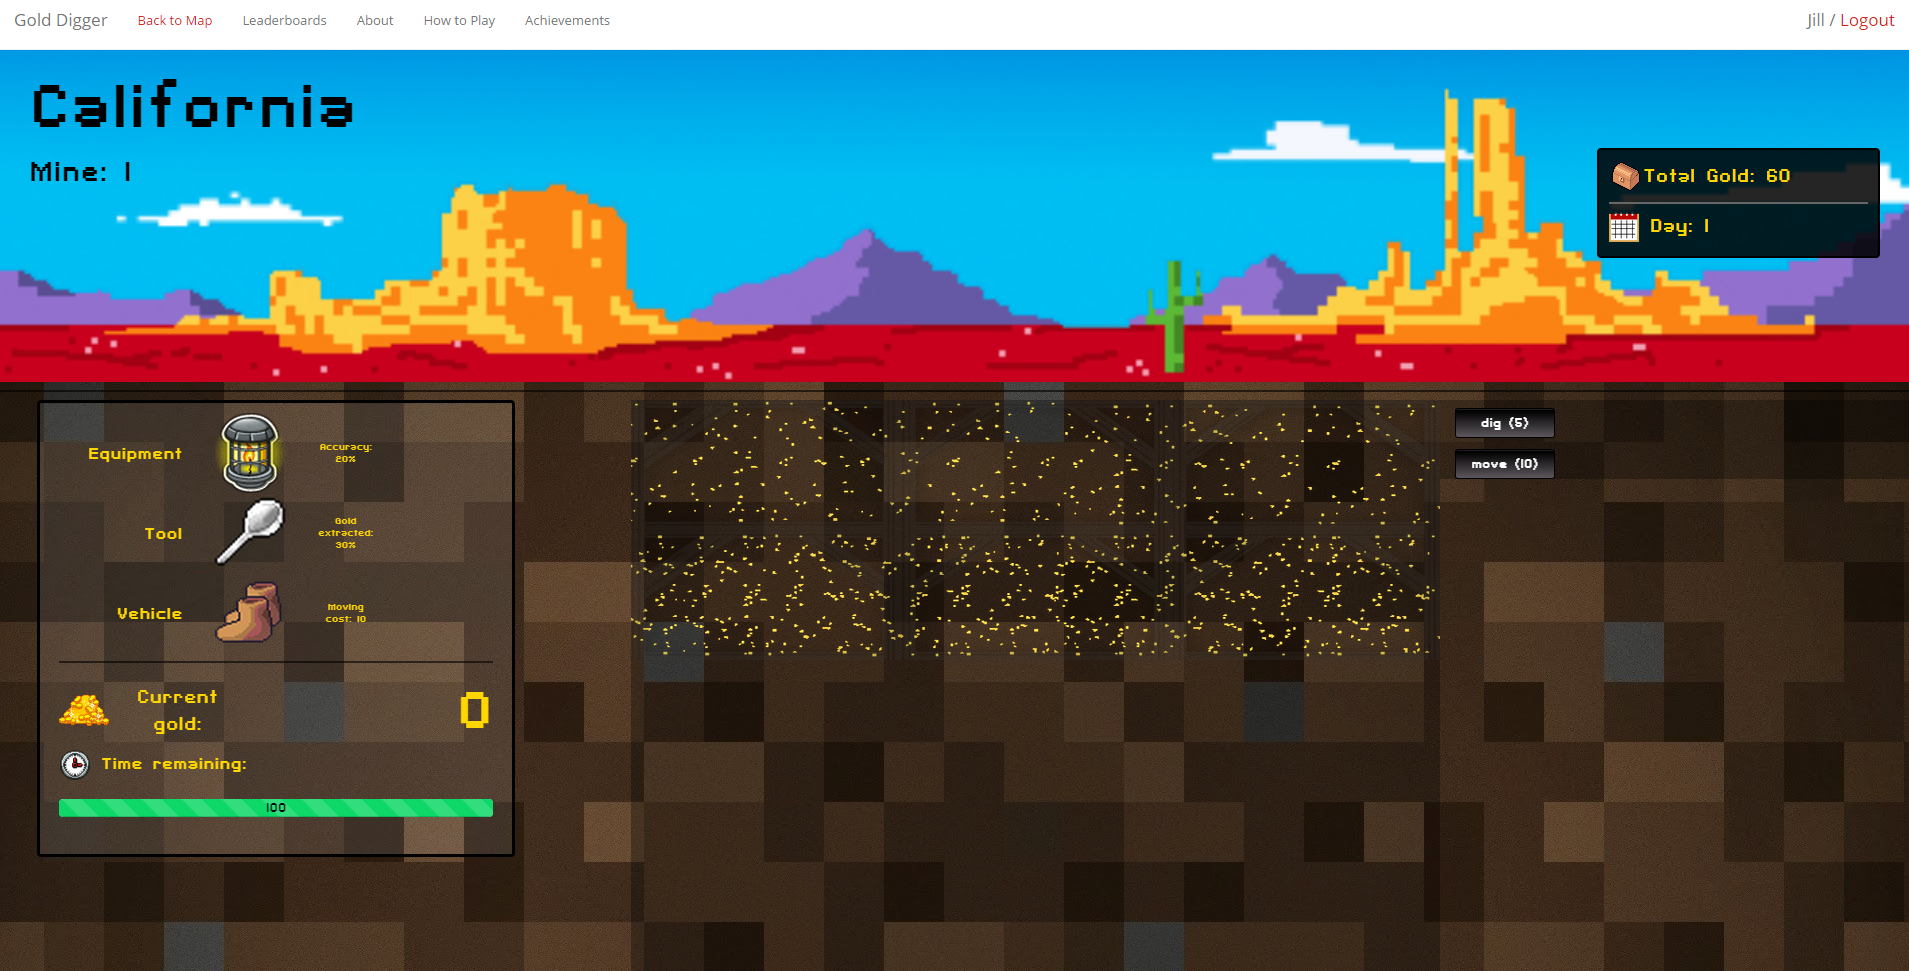
\includegraphics [width=1\textwidth] {two.png}
                \caption{The undug mine}
                \label{fig:two}
        \end{subfigure}
        \space
        \space
        \begin{subfigure} [h] {0.50\textwidth}
                \centering
                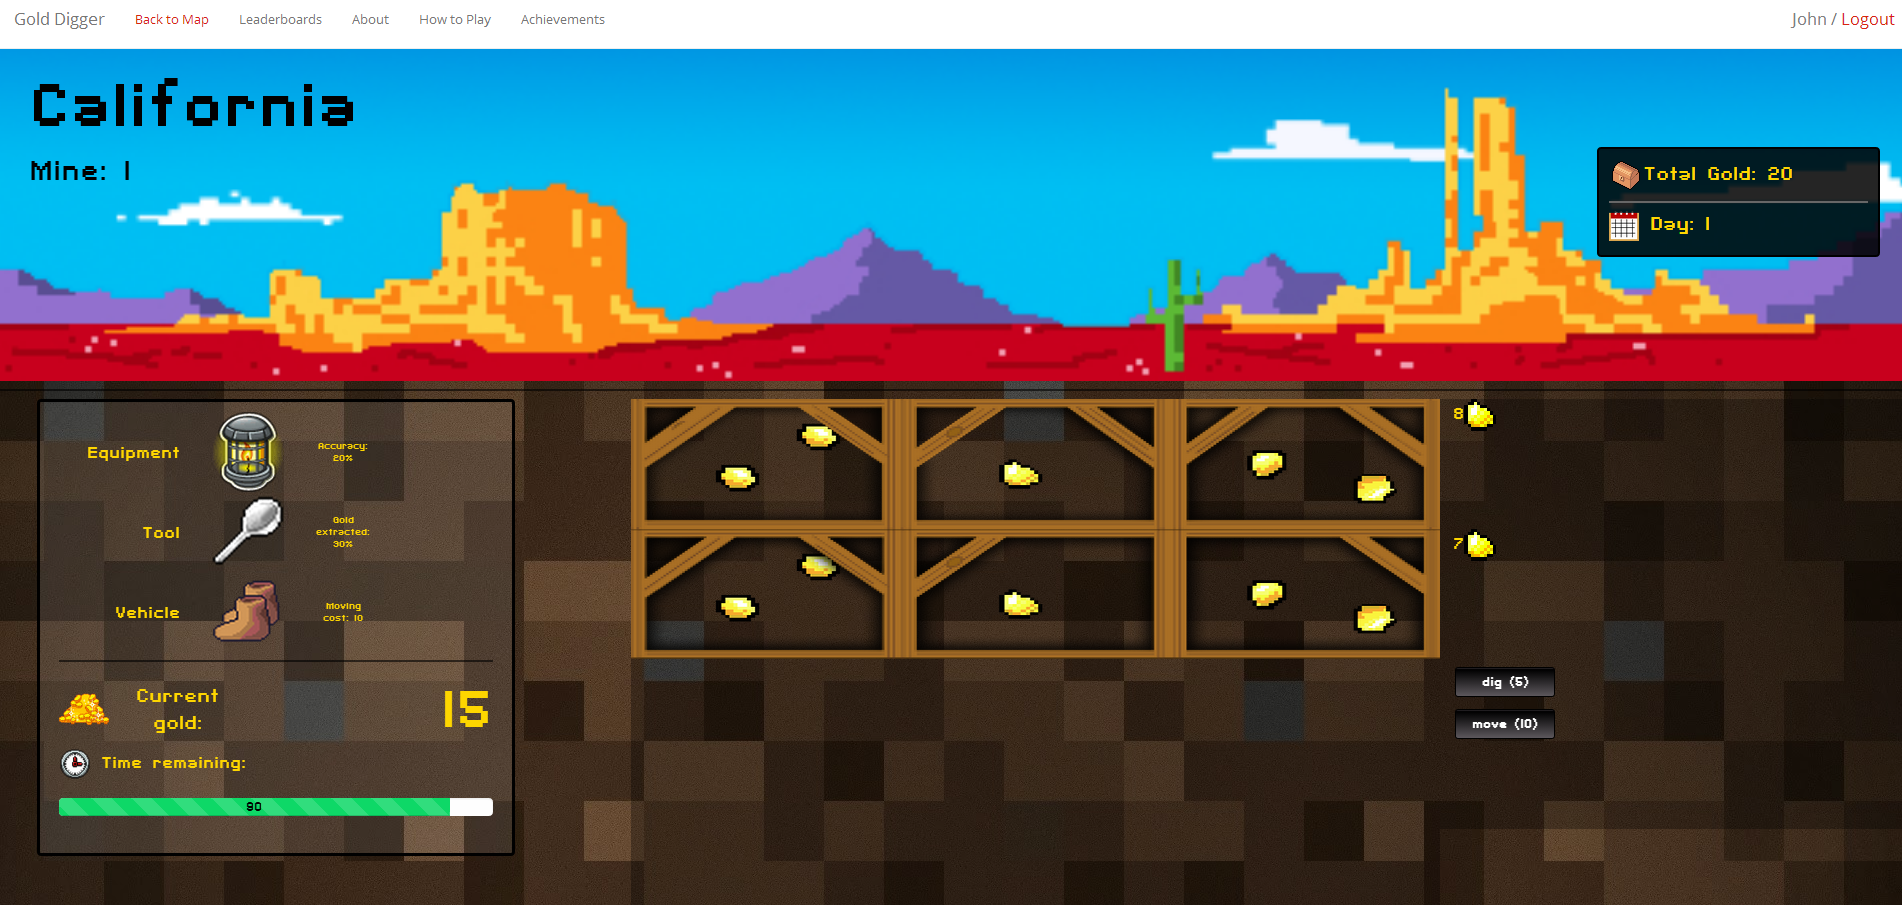
\includegraphics [width=1\textwidth] {mine.png}
                \caption{the mine has been dug twice}
                \label{fig:mine}
        \end{subfigure}
        \caption{}
        \label{fig:doublemine}
\end{figure}


(3) Jill decides to dig through the first couple of layers layer of the mine (fig~\ref{fig:mine}) by clicking on the 'Move' button on the right hand side of the mine shaft. She gains 15 gold nuggets and consumes 10 units of time (since each digging operation costs 5 units of time)
\begin{itemize}
	\item \textbf{Current gold}: 15
  	\item \textbf{Time remainingl}: 90
  	\item \textbf{Mine}: 1
	\item \textbf{Day}: 1
\end{itemize} 


(4) At this point Jill is not sure she might get much more gold from this mine and she doesn't want to spend precious time digging through layers of the mine that she has no information about. For this reason she clicks on 'Move' to get to a new mine (in the same location). To do this she must spend 10 units of time
\begin{itemize}
	\item \textbf{Current gold}: 15
  	\item \textbf{Time remainingl}: 80
  	\item \textbf{Mine}: 2
	\item \textbf{Day}: 1
\end{itemize} 

\begin{figure}[!h]
        \centering
        \begin{subfigure} [h] {0.6\textwidth}
                \centering
                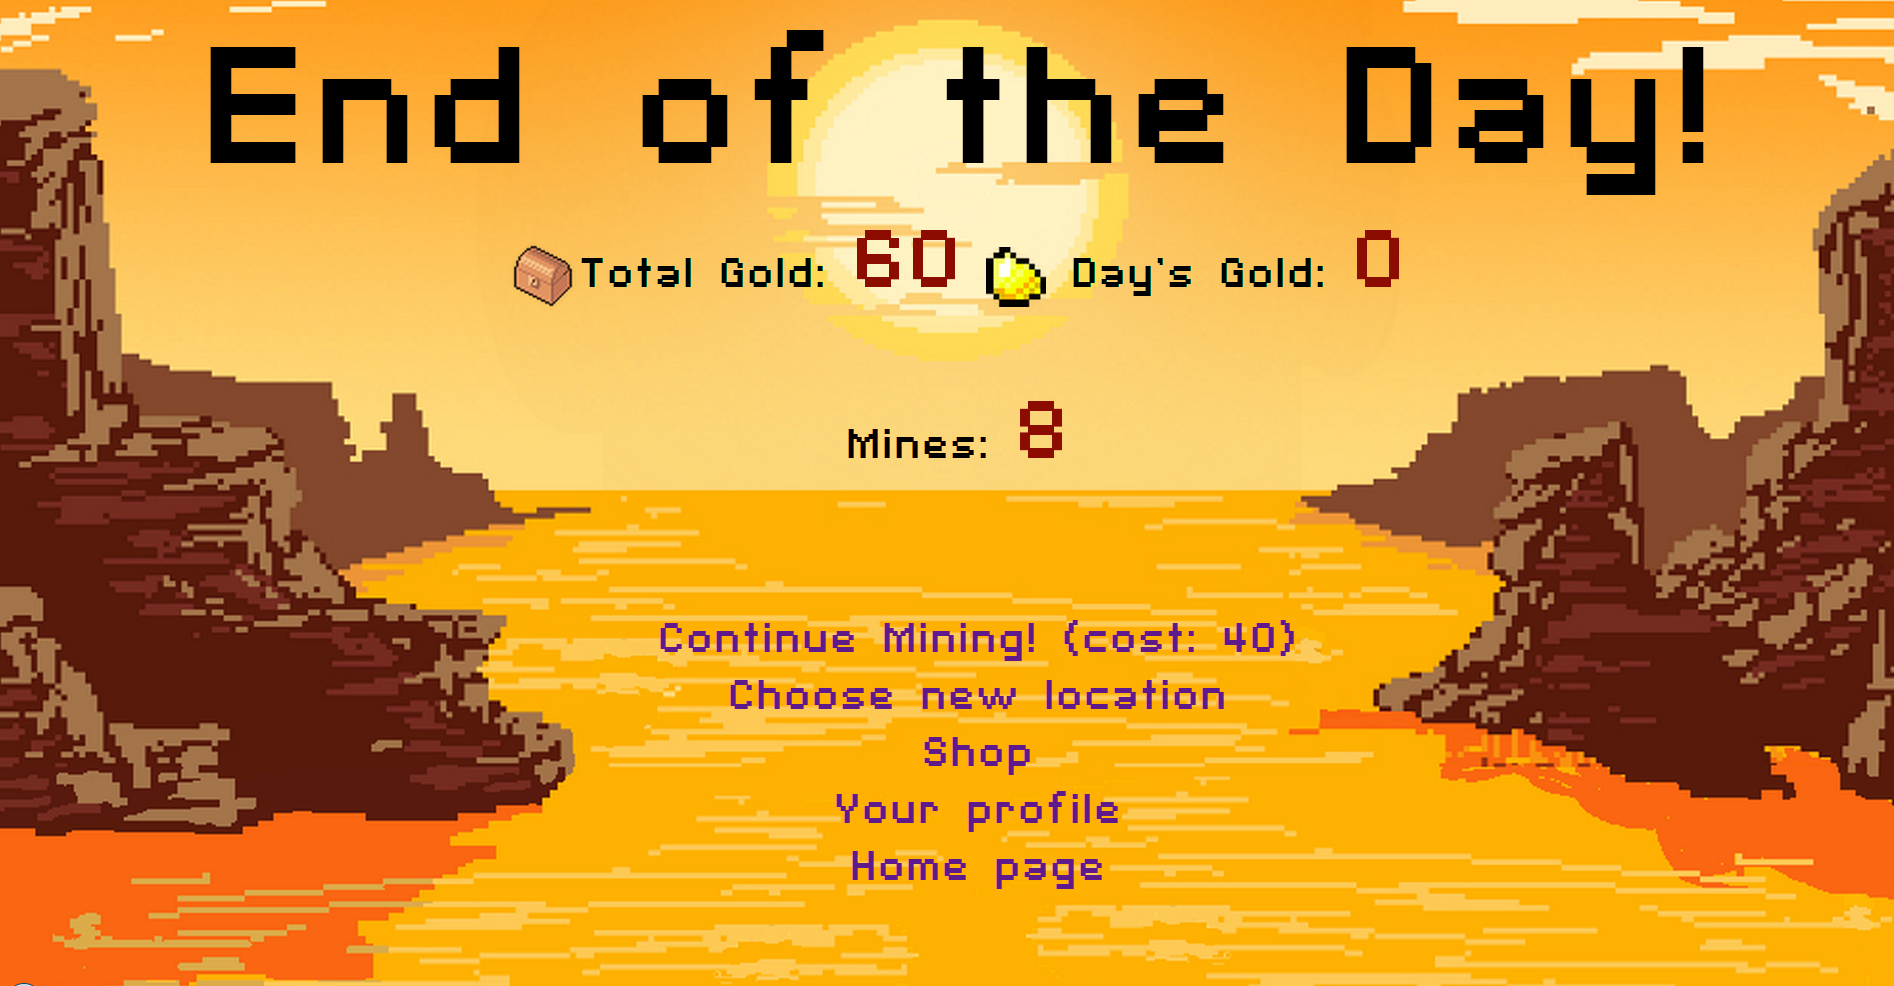
\includegraphics [width=1\textwidth] {endofday.png}
        \end{subfigure}
        \space
        \space
        \begin{subfigure} [h] {0.2\textwidth}
                \centering
                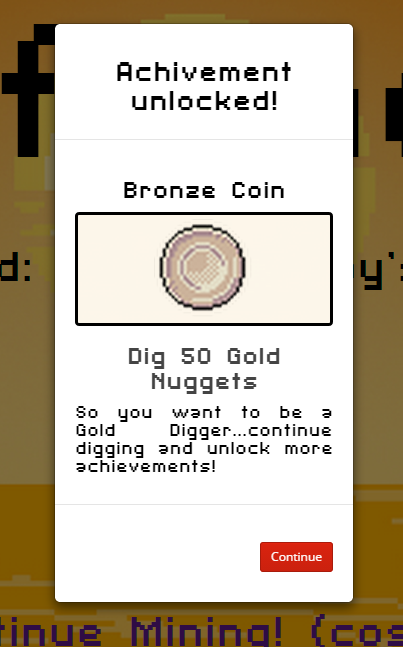
\includegraphics [width=1\textwidth] {bronze.png}
        \end{subfigure}
\end{figure}

(5) Jill continues to dig through some more mines and after a while she runs out of units of time. At this point, she is presented with the 'End of the Day' screen that sums up her progress during the day as follows:
\begin{itemize}
	\item \textbf{Today's gold}: 94 
  	\item \textbf{Total gold}: 94
  	\item \textbf{Mines dug}: 6 
\end{itemize} 
Jill also receives the 'Bronze Coin' achievement for having dug more than 50 gold nuggets. From here Jill decides to go to the shop and see if she can purchase some new items

\begin{figure}[!h]
        \centering
        \begin{subfigure} [h] {0.6\textwidth}
                \centering
                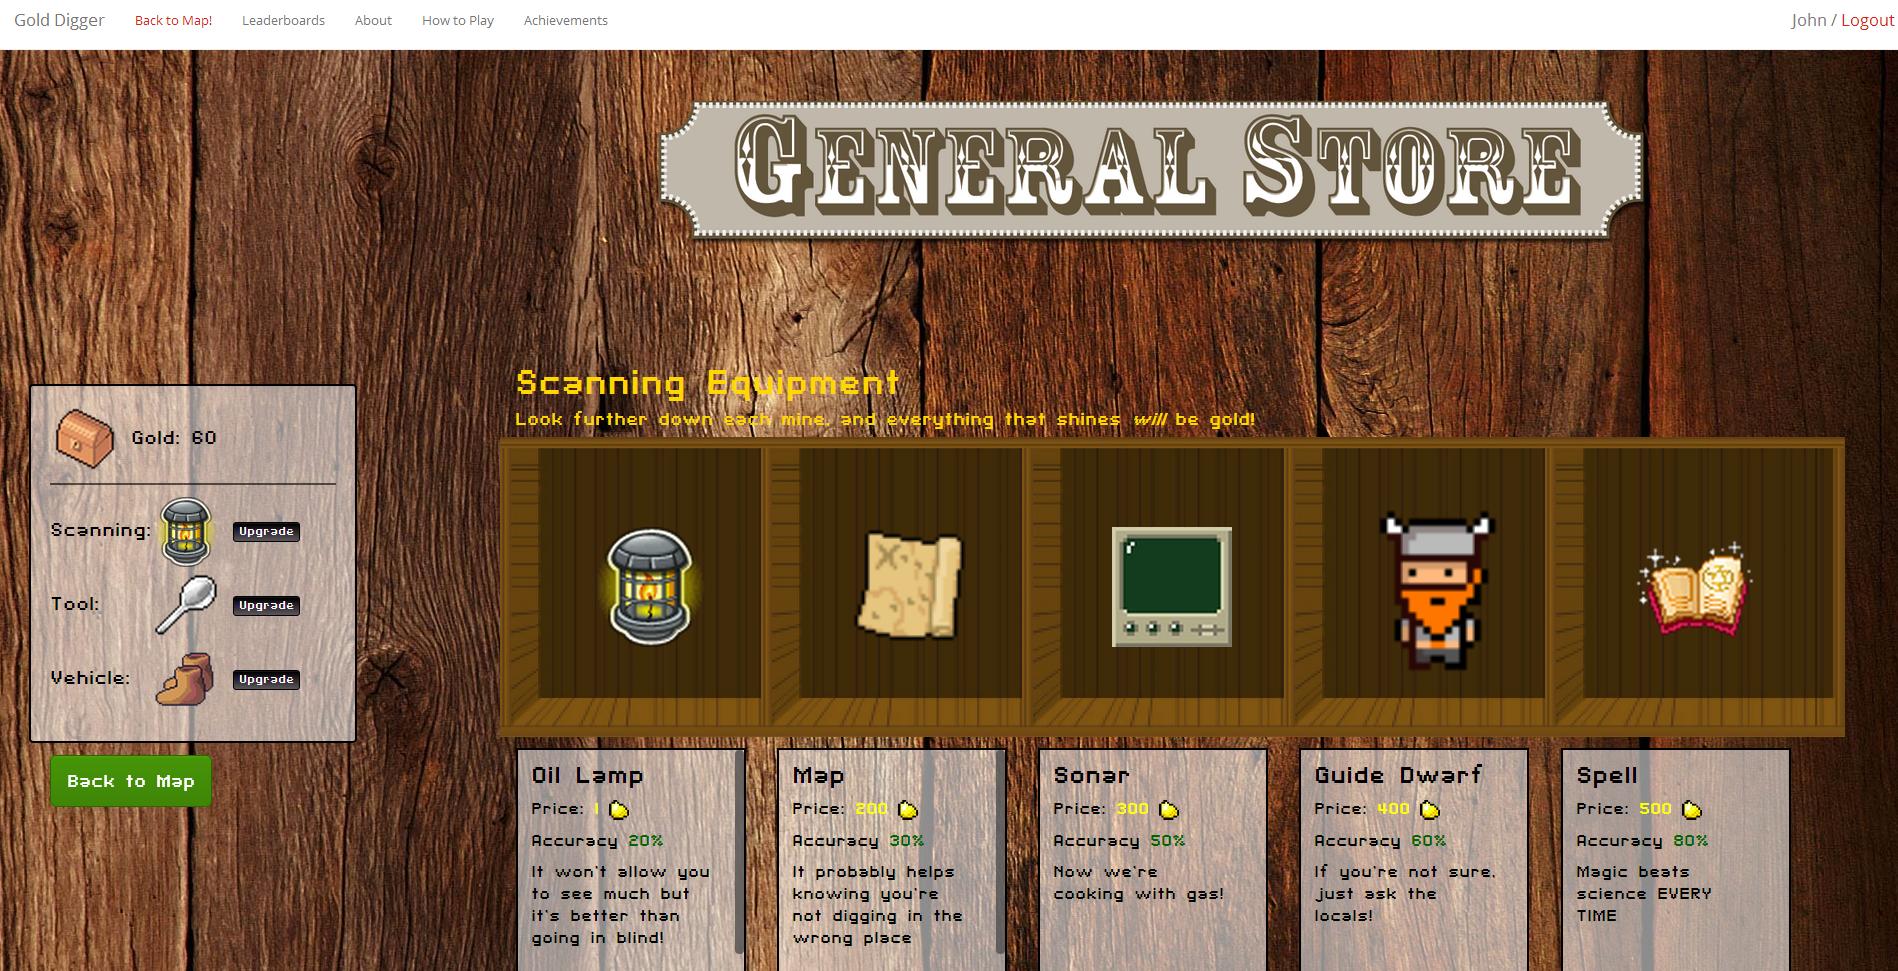
\includegraphics [width=1\textwidth] {generalstore.png}
        \end{subfigure}
        \space
        \space
        \begin{subfigure} [h] {0.3\textwidth}
                \centering
                
\includegraphics [width=1\textwidth] {nogold.png}
        \end{subfigure}
\end{figure}

(6) Once in the shop Jill tries to purchase better scanning equipment, so she clicks on the 'Upgrade' button next to the Oil Lamp. Unfortunately she doesn't have enough gold to make this purchase yet, so a message alerts her that she would need to do some more mining if she wants to be able to purchase the item.

\begin{figure}[!h]
        \centering
        \begin{subfigure} [h] {0.6\textwidth}
                \centering
                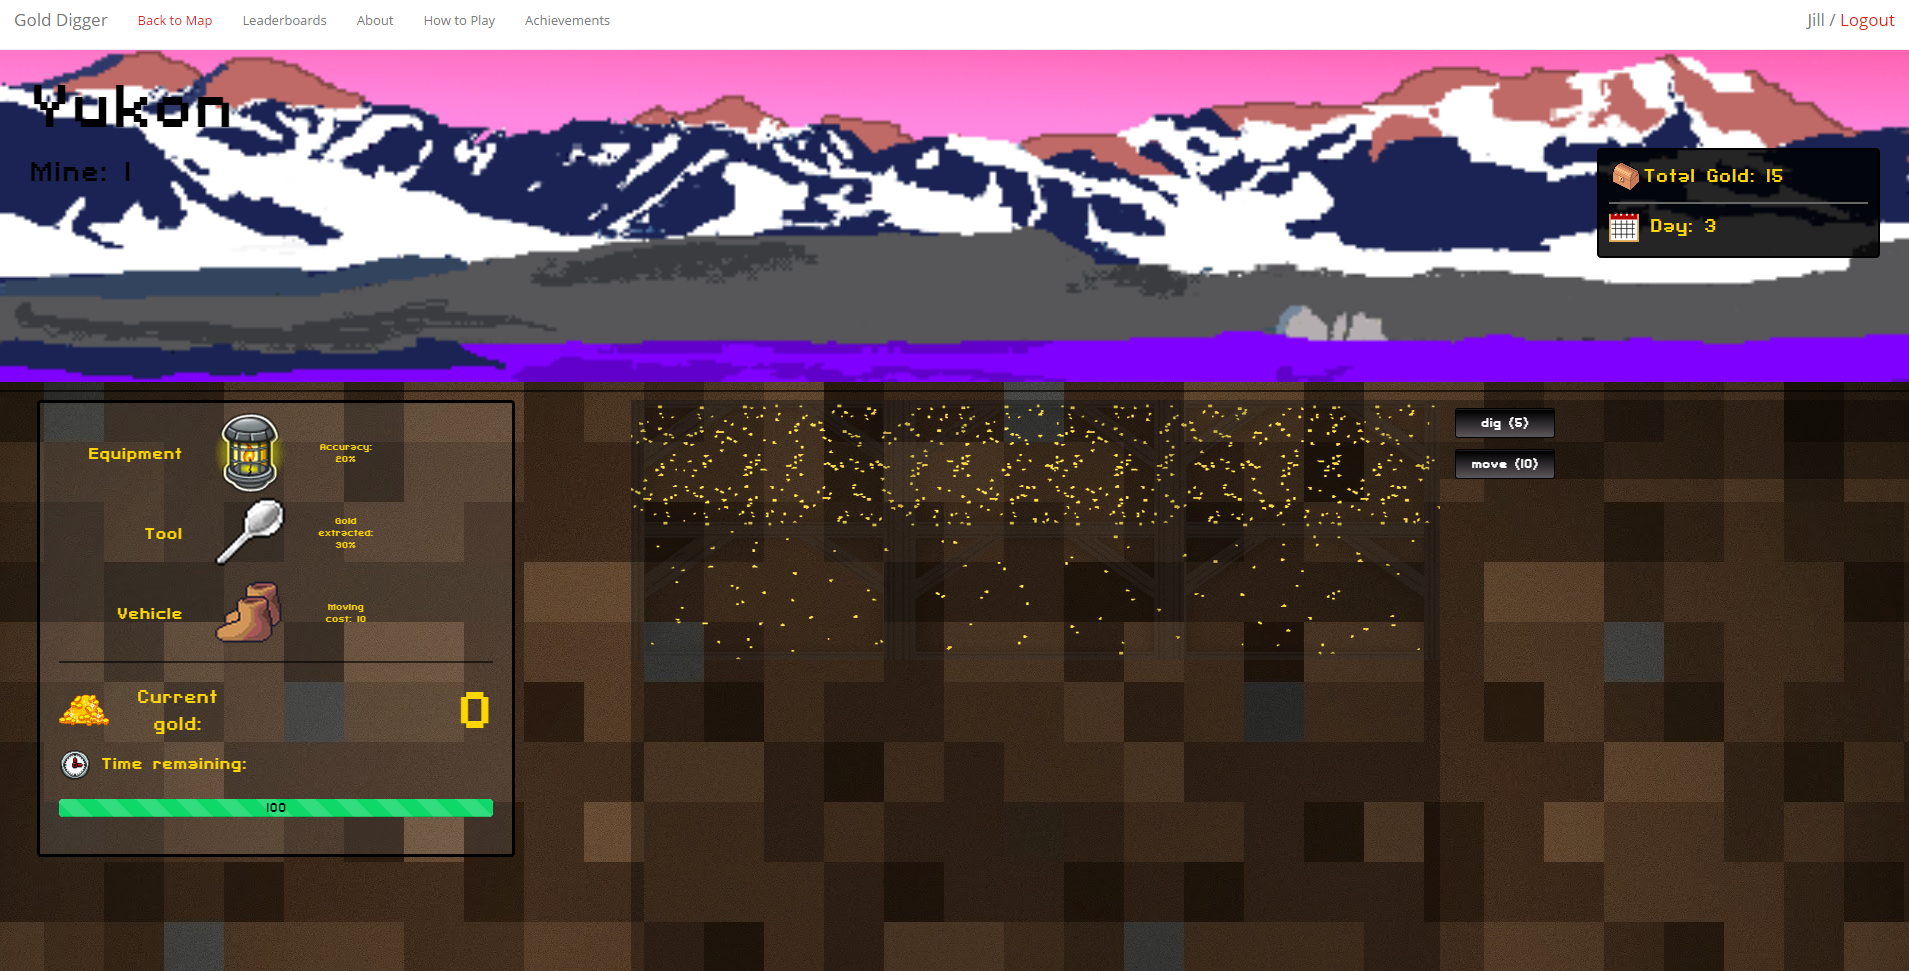
\includegraphics [width=1\textwidth] {yukon.png}
        \end{subfigure}
        \space
        \space
        \begin{subfigure} [h] {0.3\textwidth}
                \centering
                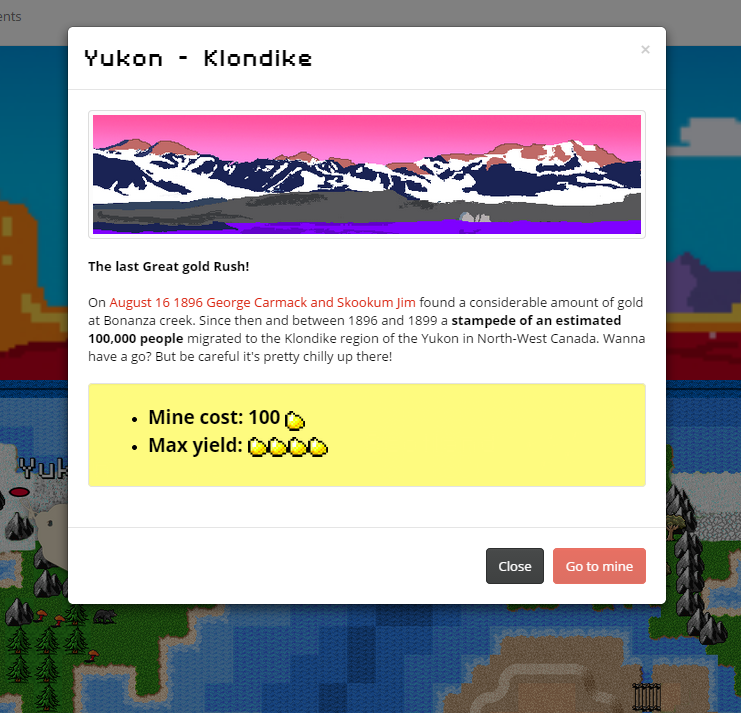
\includegraphics [width=1\textwidth] {yuki.png}
        \end{subfigure}
\end{figure}

(7) To gather more gold, Jill goes back to the California mines and, as soon as she has 100 gold nuggets, she takes a gamble and spends them on accessing the Yukon mine. However, she doesn't perform very well and, at the end of the day she owns less than 40 gold nuggets.
\begin{figure} [h] 
	\centering
           \makebox[\textwidth][c]{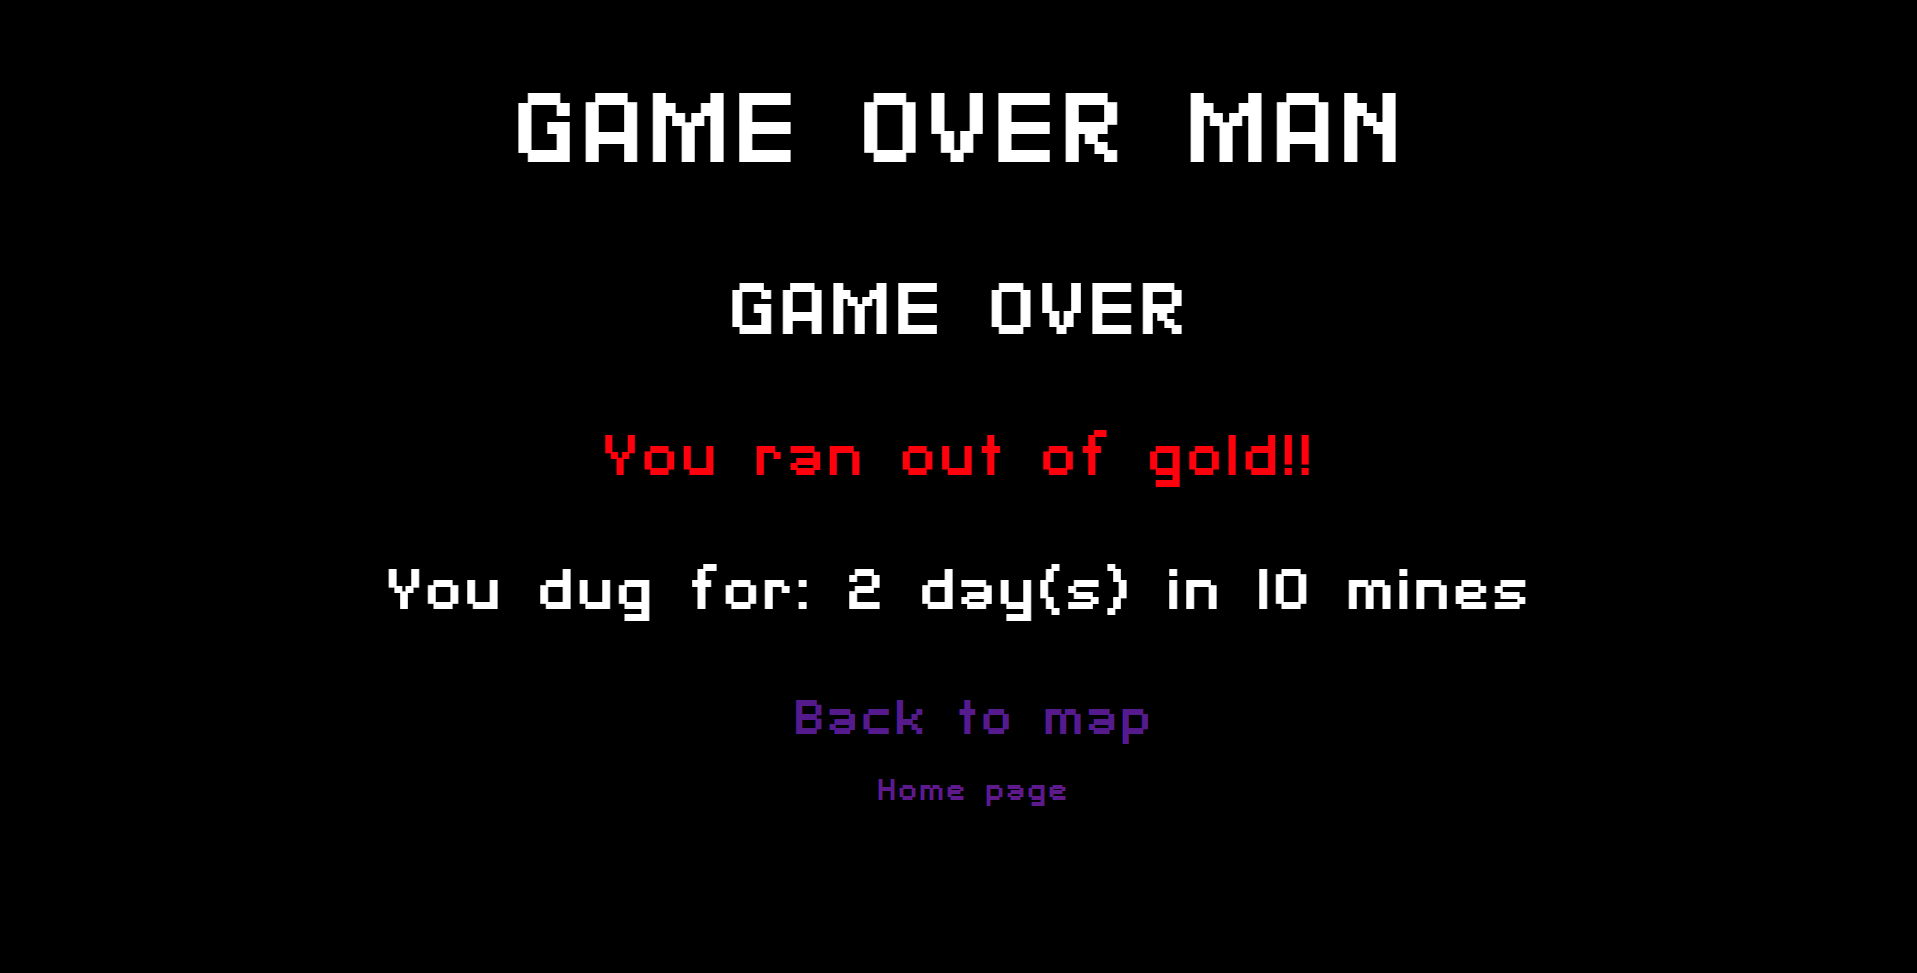
\includegraphics[width=1\textwidth]{gameover.png}}
\end{figure}
Because she doesn't have enough money to enter any of the mine, Jill loses her first game. However, clicking on 'Back to Map' will restore her to the initial conditions, if she bought any items they wold be lost.


\section{System Architechture}

\begin{figure} [h] 
	\centering
           \makebox[\textwidth][c]{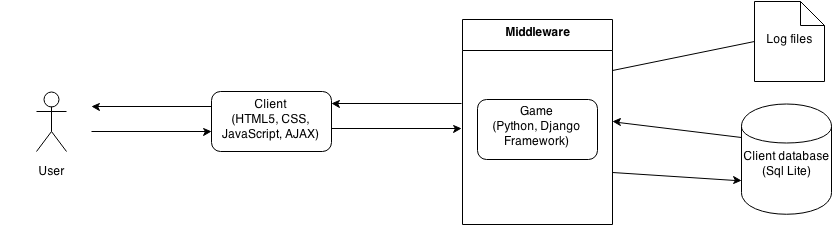
\includegraphics[width=1\textwidth]{architecture.png}}
           \caption{Gold Digger's System Architecture}
\end{figure}

Gold Digger is based on a 3-tier architecture. Each user is able to create a player account (client) containing all of the details entered upon registration, together with a set of game variables, set to their starting values. The client side renders HTML5 and CSS3 elements and graphics while updates to the game states are done mostly through AJAX, in order to avoid reloading the page. The game logic is coded in the middleware using the python-based Django framework (see \ref {subsec:Django}). All of the user profiles as well as the other game objects and achievements are stored in the database while the corresponding graphics, as well as the rest of the game graphics are stored in the project's static and media folders. Finally, the middleware continuously updates a log file in order to monitor user behaviour and gather data to be parsed and analysed at a later stage.
\section{ER Model}
\label{sec:ER}
\begin{figure} [ht] 
	\centering
           \makebox[\textwidth][c]{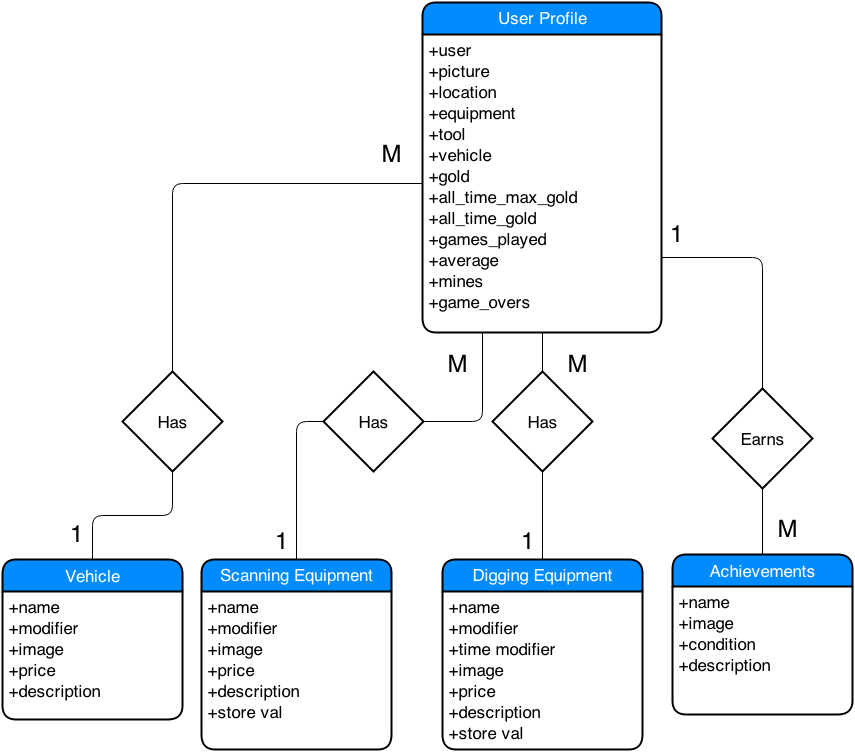
\includegraphics[width=0.7\textwidth]{er.png}}
	\caption{The Gold Digger ER diagram}
\end{figure}

The above diagram describes the entity-relationship model for Gold Digger. There are 5 entities in Gold Digger:
\begin{itemize}
	\item \textbf{User Profiles}: this entity contains several of the users' game stats, like the amount of gold at their disposal and the average amount of gold dug per mine as well as a reference to the Django object 'user' containing all the information regarding the user's password, username and email. This is necessary in order to take advantage of Django's very efficient user management system and keep the website as safe as possible 

  	\item \textbf{Digging Equipment}: this entity contains each of the tools' name, image, price and description. However, the most important attributes of this entity are the \textit{modifier} and the \textit{time modifier}. The\textit{modifier} attribute is used by the game mechanics to calculate how much gold a user is able to extract from a given layer of the mine. It is a \textit{float} number between 0.2 and 0.8  that will be multiplied by each of the amounts of gold in each layer. This way if the user is using, for instance, a shovel, she will be able to extract only 30\% of the gold that is actually present in that layer (see \ref{subsec:code}). The \textit{time modifier} attribute, on the other hand stores the digging cost per digging operation of each of the tools and it is an integer that goes from 5 to 1 in decreasing order from the worst tool to the best.

  	\item \textbf{Scanning Equipment}: this entity is quite similar to Digging Equipment but it does not include the \textit{time modifier} attribute. The \textit{modifier} attribute of this entity is responsible for calculating the cue array, that is in turn responsible for determining the amount of gold flecks that will be shown in each of the mine's layers (see \ref{subsec:code}). Furthermore, because this attribute holds only float values from 0.2 to 0.8, a simple multiplication by 10 is used  to determine the number of layers in which those specs are actually visible  .

	\item \textbf{Vehicles}: this entity, like Scanning Equipment, only posses the  \textit{modifier} attribute. This is an integer in range 10 to 6 and it holds the value of time units to be subtracted from the day's time, for each digging operation.  
	\item \textbf{Achievements}: the Achievement entity simply stores the name, image, condition and description of each of the achievements.
\end{itemize} 

\textbf{Relations}

There are \textbf{four relations} between the above entities. Each player can only store only one relation to a particular Scanning Equipment, Digging Equipment and Vehicle object thus, these are all one-to-one relationships. However, because each user can earn many achievements, the relationship between the User Profile and the Achievement entity needs a separate database table to keep track of the user-achievement value couples. In this table, \textbf{User Achievements}, each row comprises two columns, each of which is a foreign key. The first one is the relation to a User Profile Object, and the second one is the relation to an Achievement object.   

\section{Graphics}

One of the main elements of the design of Gold Digger was its graphic design. The general idea was to reproduce the look and feel of a retro 8-bit game as much as possible, without compromising the clarity and ease of use needed by a website. For this reason, 8-bit-style graphics were employed in most of the elements of the 'game pages' while Twitter Bootstrap was used in order to provide a simple minimalistic "framework" for the graphics to be displayed in. 

\textbf{Fonts}

There are two fonts that have been used throughout Gold Digger. The first one is \textbf{Open Sans} (see \ref{subsec:boot}). This font is part of the Twitter Bootstrap theme that provides the graphic framework for the site. It is used in areas with lots of text and in the navbar, where clarity the most important issue. However, throughout the site, most of the headings, scores, descriptions and game messages employ the font \textbf{SF Pixelate} (by ShyFonts) which has a pixelated look reminiscent of retro 8-bit games. All of the text in the 'game pages' is typed using this font. 

\textbf{Landscapes and World Map}

There are six different landscapes in Gold Digger, each one associated with one of the locations that the user can travel to and dig into. Three of them (California, Scotland and Yukon) were created with a pixel-art specific (Pixen) program using a number of pictures for inspiration, while the remaining three have been produced by applying filters, modifying and coloring similar pre-existing pictures in Photoshop CS, to achieve the 'pixelated look'. 

The World Map was created by importing a set of freeware game tiles into a freeware level design tool called 'Tiled' (see appendix \ref{app: firstapp}). This tool allow users to load a particular set of tiles and arrange them on a grid of their choosing. The tileset used for the World Map was originally created for the expansion and creation of new maps for the game "Tales of Middle Earth" but it lent itself very well to the task of creating a word map. After the first version of the map was completed, the location names and price tags were added with Photoshop CS 6 where other minor adjustments were also made.

\textbf{Items and Achievements}

Most of the items and achievements icons were made by Alis, a pixel artist who made them available for public usage (see appendix \ref{app: firstapp}). However a minor percentage of the items were created by modifying sprites of the popular game METAL SLUG  by SNK/Playmore. These sprites are all properties of their respective owners and no copyright is claimed upon them. 


%%%%%%%%%%%%%%%%%%%%%%%%%%%%%%%%%%%%%%%%%%%%%%%%%%%%%%%%%%%%%%%%%%%
\chapter{Impementation}
\label{implementation}

\section{Development Methods}

For the development of this project we adopted the \textbf{agile methodology} introduced by Beck, Kent et al. This methodology works by iterating through numerous cycles of development-evaluation-improvement of several working prototypes. Once the first prototype is brought to the table, a process of heuristic evaluation begins. Here the prototype is evaluated, suggestions for improvements are made and objective for further iterations are set. Then, a new cycle begins. The evaluators' feedback can also be complemented by unit and live testing. 

During the development, Gold Digger has gone through numerous cycles of development-evaluation-improvement. Every week the prototype has been discussed tested and evaluated. Then, towards the end of the project. External users were asked to play the game to outline further improvements. In this stage we were able to do most of the game balancing and design adjustments, as well as minor changes in spelling and color. We believe that the project has benefitted greatly from this kind of methodology also because of the amount of challenges we faced in development and the amount of new technologies that had to be employed. With this top-down approach, however, we were able to deliver a finished product that meets most of the expectations.

\section{Heuristic Evaluation}
Most of the improvements made to the system in its various iterations were made thanks to the technique of Heuristic Evaluation. This technique is outlined by Neilsen and Molich and represents an "informal method of heuristic analysis" that finds its strength in the amount of evaluators of the system and the number of iterations through the development-evaluation-improvement cycle. This is possible since each evaluator bring its own point of view and analysis to the table, highlighting issues that might escape each one of them if taken singularly. Neilsen and Molich define a set of metrics to evaluate a system. Here we proceed in presenting them in relation to the development of Gold Digger. 

\begin{itemize}
  \item[]{ \textbf{Visibility of system status}: the user has to be as aware as possible of the status of the system and about what's going on through appropriate feedback. In the earlier phases of gold digger, the game screen was lacking crucial information about the game status that was necessary for the user to make decisions on how to proceed playing. Two of the main variable that always need to be show to the user are the amount of gold gathered during a particular day and the time remaining before the end of that day. To visualise the firs one clearly we positioned a large counter on the left of the mine that is updated in a videogame-like 'scrolling' fashion at every dig, so that the user is always aware of the amount of gold that he is extracting as opposed to a static counter that simply jumps to the new amount. For the second one, we added a progress bar, so that the user is aware of how much time she has left at a glance.}
  \item[] {\textbf{Match between system and the real world}: users have to find themselves in a familiar environment that uses understandable vocabulary and conventions. In Gold Digger, colloquial language is used throughout. This is done not only in order for the user's understanding, but also to conform to expectations of a playful environment as it would be expected from a game. On the same lines, every effort has been made to provide the user with a familiar gaming experience that would not be hampered by the challenges of web development. To this purpose, we made extensive use of AJAX, so that we could minimise the amount of pages to be displayed.}
  \item[]{ \textbf{User control and freedom}: users should have the maximum freedom possible while navigating the system, they should never be lead to situations in which they cannot perform familiar operations. A major problem in the development of Gold Digger, has been the handling of the 'back button' and 'reload' function offered by web browsers. For instance, users might try to reload the page, try to go back or leave the game page if they feel like they've made a mistake while digging in a mine. This created a series of problems. For example, if the page is reloaded and a new mine is generated, the user has reached a new mine without paying the moving cost. For this reason, we implemented session variables that would remain the same even when the page is reloaded. }
    \item[]{\textbf{Consistency and standars}: the system should follow platform convetions, the user should not have to wonder about the meaning of terms. As stated above, every effort has been put into making Gold Digger a familiar gaming experience. All of the actions performed during play have the expected results and during navigation of non-game pages, the user is presented with a standard web site. Finally the addition of the left side item panel contributes to the consistency of the gaming experience, since it is only displayed when the user is logged in and reminds her of her stats.}
    \item[]{\textbf{Error prevention}: the system should designed in a way that makes raising error messages very rare. As mentioned in the section on User Control and Freedom, one of the main concerns has been maintaining the consistency of the present game object. However, when this cannot be achieved through session variables, the user is presented with messages alerting her of the consequences of some actions. For example, if the user tries to leave the game page, a message is displayed warning her that she will lose all her gold but that she can leave if she so desires.}
\item[]{\textbf{Recognition rather than recall}: objects, actions and options should be as visible to the user as possible, the user should not need to remember particular details if they can be easily shown. During gameplay, all of the relevant game stats are placed in the left side panel. The current amount of gold, the time remaining and the equipment are all clearly displayed and visible at a glance. The panel follows the user as she travels down the mine and, when she digs, the scroll position of the page is automatically adjusted to display the first undug layer}
\item[]{\textbf{Flexibility and efficiency to use}: following feedback from the members of the research groups, further improvements were made build upon the features discussed in the "Recognition rather than recall" sections which further enhance user experience and streamline the access to the game. First of all, upon login or registration, the user is automatically redirected to the world map so that she can immediately start playing. Secondly, a brief explanation on how the game works has been added to the main page to allow users to both evaluate the game and quickly grasp its mechanics at first glance right from the beginning.}
\item[]{\textbf{Aesthetic and minimalistic design}: every effort has been made to remove unnecessary information from each page and give the user a spacious environment to interact with. A nav bar has been imlemented at the top of each page to offer a common thread connecting all pages and at the same time occupy as little space as possible.}
\item[]{\textbf{Help user recognise, diagnose and recover from errors}: as discussed above alert messages are displayed to the user in colloquial language whenever the user tries to leave the page or purchase an object that she cannot afford.}
\item[]{\textbf{Help documentation}: this has been achieved in two main areas. The first one is letting the user know about the terms and conditions as well as the purpose of the web app. This is done upon registration or redirection to the "About" page. The second one is a tutorial that provides a clear walkthrough of the main game screen explaining all the relevant items, actions and variable that the user will be presented with.}
\end{itemize}


\section{Technologies}

\subsection{Python}
\label{subsec:python}

Python is one of the most popular programming languages with great features such as a clear syntax and an extensive amount of documentation, libraries and native methods.
The choice of using Python as a main programming language was very much tied to the web development framework chosen (Django). Nevertheless, Python has many advantages of its own, that became very important to the development of Gold Digger.  Built in methods, such as \textit{random.randint()} (to generate random integers) and \textit{pow()} (for exponentiation) were of great help in the the development of the yield functions for each mine. Furthermore, thanks to the \textit{list} object, it is very easy to create, manipulate, sort and modify both arrays and list, which proved very useful, given the structure of each mine. Finally, Python dictionaries, allow us to store pairs of values and retrieve them seamlessly in just a few lines of code which, given the number of variables each game object has to handle, is a great advantage, since then we don't need to handle handle them one by one.

\subsection{Django}
\label{subsec:Django}
Django is a very powerful, well documented, easy to use, extensive web development framework based on python. In Gold Digger, it provides the base on which all of the other technologies employed are built upon. The choice of Django as a web development framework has been made for all the reasons listed above, but some were important in particular. Firstly, Django uses a Model View Template architecture. Each url request is handled by the Model middleware in Django and redirected to a specific View associated with it. The view, in turn, handles the request and provides the data to be passed to a the Template that further processes it and diSplays it (see below for Django template code). %%%
Another one of Django's main features is the handling of SQLite databases through simple python commands. Because each user is associated with a User Profile object, frequent update of the database was needed in order to update all the game values and player stats. In Django, this is very easy and intuitive and accessing the database data can be done in any of the views seamlessly.

Furthermore, Django offers a template support through the use of \textbf{Django tags}. These Django-specific commands are enclosed in special \textbf{\{\% ...\%\}} tags and allow the advanced display of content and values sent from the views in HTML documents. Finally, Django offers session support, an easy login module, and a media server, which are all involved in the development and  functioning of Gold Digger


\subsection{HTML5}

HTML5 is the most common markup language for presenting content on the web. All of the elements of each page (visible and not) are defined by HTML5 tags, creating a structure in which content can then be easily styled thanks to CSS3 stylesheets and manipulated using Django tags (see \ref{subsec:Django}) AJAX calls (see \ref{subsec:AJAX}) and JQuery. Two of the most important HTML5 attributes, are the \textbf{class} and \textbf{id} attributes. Classes allow similar elements to have the same style, thus allowing us to maintain integrity of graphics throughout the website without having to modify the paramentes of every single element. Elements with the same classes will exhibit similar properties. Finally, the  \textbf{id} attribute, allows us to refer to particular elements when we want to modify or alter them in some way using technologies such as AJAX and JQuery (see \ref{subsec:JS})

\subsection{CSS3}
\label{subsec:CSS3}
As mentioned in the previous section, styling is applied to HTML5 elements via reference to CSS3 stylesheets. In CSS3 sheets we can define the parameters for the styling of each class, id or element that is present in one of the templates. If a template displays a link to a particular stylesheet, elements that display one of the classes defined in that stylesheet, will be formatted accordingly. In the example below, we can see how styling is applied to the element with id 'home': 

\lstinputlisting[language=HTML, firstline=4, lastline=12]{custom.css}

here, a background picture for the homepage heading is defined and set in place using the \textit{padding} parameters.Padding is one of the parameters for positioning and styling elements of that are associated with the HTML box model.

Finally, CSS3 is indispensable in order to implement web page's responsiveness, in order for the pages to be displayed appropriately on screens of different sizes. There is more than one technique to make this possible but, in Gold Digger, we used \textbf{media tags} which specify the styling of particular items for different screen size ranges.

\textbf{Animate.css}
\\
\\
In addition to offering the possibility to style HTML5 elements, CSS3 also offers the possibility to apply animations to them. The Animate.css library (by Daniel T. Eden) in particular, makes this as easy as adding the 'animated' class to any element we wish to apply an animation to, together with an attribute defining the kind of animation. These animations are used mainly in the mines, to make each layer of  scaffolding in the mine appear by descending from the top, as well as nicely presenting the new mine when it's first created. Since Gold Digger is fundamentally a video game, and since one of video games' fundamental features are their animations, it seemed non trivial to add some animated element to match user's expectations on this matter. Animate.css allows us to do this easily and cleanly.

\subsection{Twitter Bootstrap CSS}
\label{subsec:boot}

Twitter Bootstrap uses a both CSS3 and Javascript to offer the possibility to apply sleek and minimalistic themes to webpages that implement a link to them. The theme used for Gold Digger, is '\textbf{Simplex}'  (by Thomas Park for Bootswatch) and it has been very useful for the organization and styling of the many elements of each page. Firstly, Bootstrap offers a very easy to use grid system, that allows us to easily divide any section of the page in columns and sub-columns. This can be seen throughout the website where the left side column hosts the side item panel, the middle column the main content (for example the layers of a mine) and the right column holds any additional information or just provides spacing. Secondly, Bootstrap comes equipped with Javascript plugins for the display of modals and tooltips. The former ones, for example, are used both in the world map to display the details of a location and on the main page, to host the registration form. Finally, Bootstrap allows to display continuity of colour and graphics throughout the website, since to equal elements always corresponds equal graphics.

\subsection{Javascript and JQuery}
\label{subsec:JS}

JQuery is a very useful Javascript library that allows to apply special animations and features to elements of a webpage. By writing functions that are activated upon key press, click or hover, we can make webpages even more interesting and interactive than by simply using CSS3 and Bootstrap. There are two main applications of JQuery and Javascript that contributed to the look and functionality of Gold digger.

\textbf{Trip.js}
\\
\\
Trip.js is a very useful library to implement guided tours of an web app or website. It allows developers to design explanatory labels for each of the elements of a web page, with the option of highlighting them if necessary. Trip.js also incorporates Animate.css to allow the labels to be displayed with nice, tidy animations. 

\lstinputlisting[language=Java, firstline=2, lastline=12]{tripprova.js}

Here we can see one of the labels being defined and attahced to the \#California\_landscape element, with a particular message and position. Finally, upon page load, the \textit{.start()} method is called on the Trip object (containing the array of labels) and the tour begins.

\textbf{jquery-animate-numbers.js}
\\
\\
This very simple JQuery plugin allows to animate numbers so that all the numbers in a given interval are displayed in a 'rolling' fashion. 
\begin{itemize}
  \item[] HTML
  \item[] <div id="num">1234</div>
  \item[] JS
  \item[]\$("\#num").animateNumbers(4321);
\end{itemize}
In Gold Digger, this plugin is used in any page in which the amount of gold is incremented or decremented (like in a mine or in the shop). Animating numbers, like adding animations with Animate.css also contributes to the 'game feel' necessary for Gold Digger.

\subsection{AJAX}
\label{subsec:AJAX}

AJAX stands for Asynchronous Javascript and it is an ensemble of technolgies that, together, allow a web page to exchange data with the server without having to reload the page itself. This is achieved through an extra layer of interaction between the server and the client that is known as AJAX Engine. In Gold Digger, AJAX is essential, especially in the 'game pages' in order for the user not to have a disjointed gaming experience in which the page would have to be reloaded and be re-compiled every time. AJAX is also used in the general store page, to smoothly display the new item in the side item panel, and in the assignment of achievements, to display them as soon ar they are earned. Thanks to AJAX we are able to keep the game experience close to what the user would expect while playing any other stand alone game. Since video games normally exist in a 'continuous evironment', they do not have to deal with the limitation of separating content in  different pages, however, with AJAX we are able to successfully compensate for this issue. 

\section{Development challenges}
\label{sec:dev}
Most of the development challenges we faced during the development of Gold Digger were related to the dual nature of Gold Digger. On the one hand, Gold Digger needed to be a game to experiment on searching behaviour and information retrieval, while on the other it had to be developed as a website, adding all the challenges of web development to the development of a game. Video games, even simple ones, usually exist in their own environment, in which all the variables needed can be easily accessed and modified. In a website instead, this continuity needs to be compensated for with session variables, access to user objects and above all, interaction with the database. 

Other challenges in the development of Gold Digger, were the design of the game mechanics and the implementations of the methods and functions involved in the creation of the yield a and cue arrays. These last ones needed to produce values  that, while being generated by a function, would still appear random enough to the user so as to offer a more challenging and interesting gaming experience. In the following subsections we outline some of the strategies used to overcome these challenges.
\subsection{Creating mines}
\label{subsec:creatingmines}
(1)By selecting a location from the world map, the user sets the session variable 'location' to the name of the location selected and the '\textbf{has\_mine}' parameter to an empty string. Then, the request is redirected to the \textbf{game2} view in order to initilise all the game variables

(2)The \textbf{game2} view first checks if the '\textbf{has\_mine}' variable contains an empty string (meaning that this is the first mine of the day) and then uses the 'location' previously set (see (1)) value to determine which yield generator to select to generate yields. There are six different yield generators. Each one will generate a different array of ten values, representing the amount of gold in each layer of the mine.

(3) Once we have a YieldGenerator, we need two more values to generate a mine. These are: '\textbf{accuracy}' and '\textbf{user}'. The former one contains the value of the tool's modifier which will be needed when generating cues. The latter one is needed for logging statements. By creating a \textbf{Mine} object, we automatically trigger the \textit{make\_mine()} method in the Mine class which, in turn, triggers the \textbf{make\_yields} method of the YieldGenerator thereby starting the process of generating yields.

(4) All the different yield generators inherit the \textbf{make\_yields}  method from the YieldGenerator class and define their own. This way we are able to add as many yield generators as needed, by simply adding a new method implementing  \textbf{make\_yields}. Each yield generator defines its own static function that will generate an array of yields according to a specific equation that also introduces some randomness. Below, we can see the static function in charge of determining the yield of mines in Scotland.

\lstinputlisting[language=Python, firstline=260, lastline=270]{yieldgen.py}

On line 5 we have a quadratic function generating a parabola which it takes \textbf{x},  \textbf{a},  \textbf{k} and \textbf{b}  as paramenters. The value of \textbf{x} goes from 0 to 9 and it represents each of the layers of the mine. \textbf{a} determines the steepness of the parabola and  \textbf{k} determines the position of the parabola on the x axis (see \ref{app:firstapp} for a graph representation of each mine). This function will return a value \textbf{y} for each of the values of x. Each of these values, in turn, is rounded to the nearest integer and added to the array of yields. Finally, as we can see on line 3 a certain degree of randomness is introduced with \textbf{b}, which modifies the height of the parabola and consequently each one of the yields. \textbf{k} is also a random number in a range, this way, we don't run the risk of producing the same mine over and over again. All of the static functions in each of the YieldGenerators has some degree of randomness.

(5) A cue is a number from 0 to 6 determinig which of the gold flecks patterns will be displayed over an undug layer of the mine. As we will see in the next section, each of these images is associated with a class and Django tags will use the value of 'cue' in each block to display the appropriate one. Once the array of yields is ready and has been received by \textit{make\_mine()}, it is passed to \textbf{cuegen.py} together with the value containing the highest of the yields and the 'accuracy' level we discussed in (3) in order to begin the process of determining the cue corresponding to each yield.   In \textbf{cuegen.py} we set the number of possible cue patterns, then, we go through the following operations:

\begin{itemize}
	\item{Determine the cue range: this is the maximum yield divided by the number of cue patterns. A different cue (gold flecks image) will be displayed in association with each range.}
	\item{Determine the span: this is the span in which the cue will be chosen, the wider the span, the least likely the cue displayed will match the yield. It is a function of the maximum amount of point and the accuracy of the scanning tools. In the table below, we can see an example in which the maximum yield of the yield\_array is 42. If for instance the yield is \textbf{x} and the user's scanning equipment is the lamp the cue span will be wider (orange) and any of cue the cue patterns 1 to 3 might be displayed. However, if the user is using a sonar (green), which is more accurate, the cue pattern displayed will be either 2 or 3. This way, we are able to display cues in relation to the accuracy of a user's item. The better the item, the smaller the span.}
\end{itemize}

\begin{figure} [!ht] 
	\centering
           \makebox[\textwidth][c]{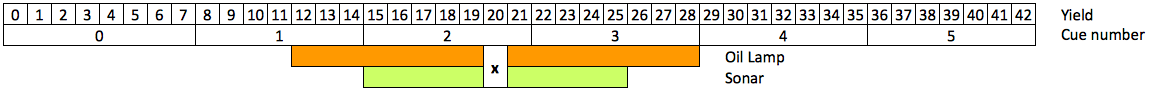
\includegraphics[width=1\textwidth]{span.png}}
           \caption{}
\end{figure}

\begin{itemize}
	\item{Choosing the cue: as discussed above, a value in the range of the cue span is chosen at random and the associated cue appended to the array of cues which is then returned to the Mine class}
\end{itemize}

(6) Now that we have both the array of yield and the array of cues, we are able to assign values to each of the \textbf{Block} objects representing each a layer of the mine. Each Block object, in fact, contains the following values:
 
 \begin{itemize}
 	\item{\textbf{pos}: the position of the mine, an integer from 0 to 9}
	\item{\textbf{gold}: the yield}
	\item{\textbf{cue}: one of the 6 cue values representing one of the patterns}
	\item{\textbf{dug}: a boolean determining if the mine has been dug or not}
\end{itemize}

(7) The array of blocks is sent over from the \textit{game2} view to the template, in a dictionary, together with all the other values relevant to the display of the game page.

\begin{figure} [ht] 
	\centering
           \makebox[\textwidth][c]{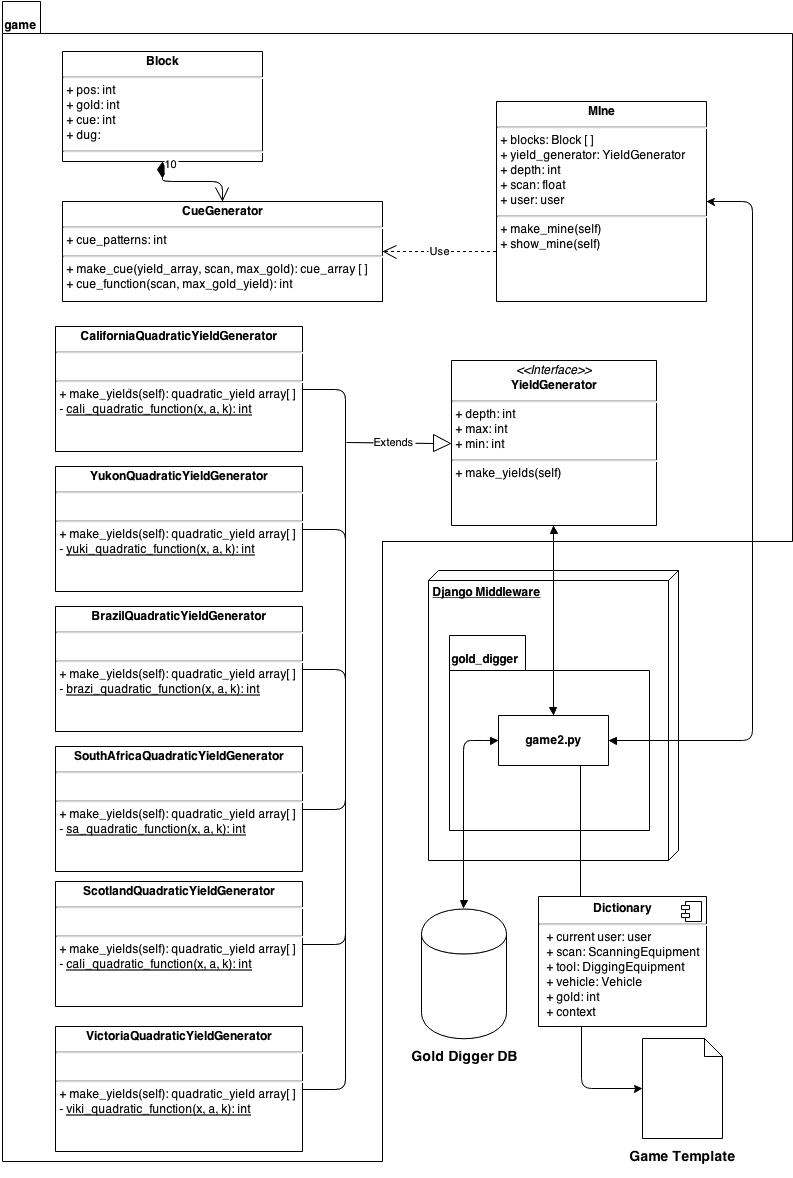
\includegraphics[width=1\textwidth]{classdiagram.png}}
	\caption{The class diagram illustrates the way the game object is prepared and sent to the template for display}
\end{figure}

\subsection{Digging: sessions AJAX}

A fundamental functionality that needed to be implemented in Gold Digger was the ability of the user to continue digging into a mine without having the page reload. When digging, a certain amount of gold is acquired, while a certain amount of time units are spent. At the same time, gold flecks layers or shaded layers of scaffolding, need to be replaced with the appropriate graphics and animations. Django helps us very much in the display of all the items needed in this process, however, once the page is rendered and displayed, we would need to reload it for any content to be altered, by redirecting to the appropriate view and get back to the template. 

The first step in addressing this problem has been the implementation of sessions. Sessions support comes pre-built in Django and it is thus very easy to take advantage of. Sessions are employed mainly in maintaining each mine constant upon digging or reloading the page. Each mine, once created and until the moment when the user decides to move away from it, needs to remain constant, this means that its gold yields would not be generated anew and that, furthermore, the user will be able to see the amount of gold harvested from the layers she already dug. 

To achieve this, we make use of two main session variables: \textbf{'pointer'} and \textbf{'pickled\_blocks'}. The 'pointer' variable is responsible for holding the value of the position of the right hand side buttons used to dig and move while the 'pickled\_blocks' variable is responsible for holding the pickled array of blocks representing the current layers of the mine. Because there are several passages involved in this mechanic it is probably helpful to break them down into steps:

(1) When the user enters a mine, the \textbf{game2} view is accessed. This view is responsible for returning a dictionary to the game template with all the values relevant to the mine and the player's status. The 'pointer' variable is set to 0, while the array of blocks representing the layers of the mine is 'pickled' (see \ref{}) in order to be added to the session values and used later. 

(2) The template receives the dictionary sent by the \textbf{game2} view and displays it with the help of Django tags. First of all, we check if the dictionary contains an array of blocks, if it does we proceed to further conditional statements to decide how each one of those blocks is going to be displayed (see below). 

(3) First of all, we check if the block has been dug or not. This is done by checking if the 'dug' parameter is True or False. Depending on the case, different graphics will be displayed.

\lstinputlisting[language=HTML, firstline=136, lastline=147]{game2.html}

In the code snippet above, we can se what happens if the 'dug' variable of a block is False. Thanks to a particular kind of Django tags (the double curly braces) we can display the appropriate cue, granted that our visibility (line 4) is greater than the number of the layer we are in at the moment. On line 6 we can se how \emph{class=row\_flecks\_\{\{ block.cue \}\}} will display a different row of flecks according to the value of \emph{\{\{  block.cue \}\}}. A similar process will take place if the 'dug' value of a block is True, except in this case we will use \emph{class=row\_nuggets\_\{\{ block.cue \}\}}, which diplays the appropriate amount of nuggets and the scaffolding of an already dug layer.

(4) Now that all the layers of the mine have been correctly displayed, we need to take care of the right side panel which hosts the game controls: the \textbf{dig} and \textbf{move} buttons. To each layer of the mine corresponds a row containing a button couple on the column to its right. However, all of them are hidden from the user except the one corresponding to the the first undug layer. Once the user clicks the \textbf{dig} button, the row is removed and the '\textbf{hidden}' attribute is removed from the row below it so that the button can be shown next to the next layer. At the same time, the amount of gold dug in the previous layer is displayed.

(5) This modification of the DOM elements properties is achieved through AJAX and JQuery. When the user clicks on the \textbf{dig} button (or Enter is pressed), an AJAX event is triggered. The number of the layer and the amount of gold that it contains are sent to \textbf{dig-ajax.js}  together with the \textit{csrf middleware token} (required by Django for security purposes) so that they can be used in the \textbf{ajaxview} view where all necessary updates to both session and database variables will be made.

\lstinputlisting[language=Python, firstline=561, lastline=563]{views.py}

Here, we can see how the session variable 'pointer' is incremented by , while  'time\_remaining' and 'gold' are updated in relation to the items possessed by the user. 

(6) In \textbf{ajaxview}, we also take care of un-pickling the array of blocks held in one of the session variables and update it. This is done in order to be able to maintain the array of blocks constituting the current mine until the user moves to a different one. If this didn't happen, the user would be able to simply reload the page and get a new mine every time at no cost. For this reason, it is very important that the array of blocks is maintained until a new mine is generated, otherwise, users who took advantage of this glitch would be able to gain an unfair advantage and the data extracted would not be reliable.  

\lstinputlisting[language=Python, firstline=541, lastline=551]{views.py}

(7) At this point, a JSON object (\textit{myResponse} containing all the necessary values is  is compiled and sent back to \textbf{dig-ajax.js} where, thanks to JQuery, we can make the appropriate modifications to update the game page.

\lstinputlisting[language=Python, firstline=592, lastline=597]{views.py}

(8) In \textbf{dig-ajax.js} we use a combination of JQuery methods and plugins in order to update the content. In the code snippet below, we can see how the elements with id 'totalgold' and currentgold' as well as the 'progress-bar' class are updated. For the first two (lines 2 and 4) we use the \textbf{.animateNumbers} (see \ref{subsec:JS}) plugin in order to make the digits 'scroll' in videogame-like way, while, for the last one (line 3) we simply use the JQuery method \textbf{.css} to change the \textit{width} attribute of the element, thus shortening the bar indicating the remaining amount of time units. Finally, in lines 6 to 8, we make sure that the scrollbar is positioned in line with the first undug layer, so that the user doesn't have to scroll down the page every time she finished digging the visible layers. 

\lstinputlisting[language=Java, firstline=72, lastline=79]{dig-ajax.js}

In a similar way, we also update the mine layers to display the appropriate amount of gold nuggets and the right scaffolding graphics. As discussed in (4), here we also take care of revealing the next layer of buttons by removing the 'hidden' class from it, while at the same time replacing the previous layer's buttons with the amount of gold dug. 

(9) In the game template, the current gold and time remaining value are updated, the gold nuggets displayed and the scaffolding brought in with an animation. If the user now decides to change mine and move, a new mine is created in the \textit{game2} view and the page is reloaded. Since in this case the digging needs to start from the top again. 
\section{Testing}
\subsection{Unit Testing}

There are several key areas in the code for Gold Digger, as we've seen in section 4.4 there are various functions that not only are fundamental to the functioning of the game, but that can modify its behaviour completely. For this reason we've implemented a series of unit tests. This way, at each stage in development, we can run the test and check that everything still works according to plan. Unit testing is another very useful Django feature which allows us to simply write tests in the \textit{tests.py} file and launch them all at the same time from the terminal. The unit tests for Gold Digger are divided in four classes, each comprising of different tests:


\begin{itemize}
	\item{\textbf{ModelTests}: this class include tests relating to Gold Digger's models.
		\begin {itemize}
			\item{\textbf{test\_user\_profile\_data}: checks if a user can be successfully added. The test fails if any of the parameters of the UserProfile model don't correspond to expectation. }
		\end{itemize}
	}
	\item{\textbf{FormTests}: this class include tests relating to Gold Digger's forms.
	\begin {itemize}
			\item{\textbf{test\_clean\_password}: checks to make sure that a user who enters a confirmation password that is different from her first password, fails authentication. }
	\end{itemize}
	}
	\item{\textbf{CueTests}: includes tests related to the appropriate generation of cue values
	\begin {itemize}
			\item{\textbf{test\_appropriate\_cue}: checks that given an array, a maximum of gold and a scan value,  \textit{cuegen.py} produces the appropriate cues. }
			\item{\textbf{test\_cue\_function}: checks that, given an array, a maximum of gold and a scan value,  \textit{cuegen.cuefunction()} produces the appropriate span values (see \ref{subsec:creatingmines}).}
		\end{itemize}
	}
	\item{\textbf{GameTests}: includes test related to the appropriate functioning of yield functions. The first six tests were developed in the first stages of the development of Gold Digger. They test six YieldGenerators that are not used in the present version. However, we made the decision to keep them in case future development demands for the use (and testing) of those YieldGenerators. The following tests were developed in order to test the presently used YieldGenerators as well as the creation of a mine. 
	\begin {itemize}
			\item{\textbf{test\_constant\_yield}}
			\item{\textbf{test\_random\_yield}}
			\item{\textbf{test\_linear\_yield}}
			\item{\textbf{test\_cubic\_yield}}
			\item{\textbf{test\_exponential\_yield}}
			\item{\textbf{test\_quadratic\_yield}}
			\item{\textbf{test\_positive}: beacuse the YieldGenerators used in the most recent iteration of Gold Digger generate yield according to functions which are somewhat randomized, it is difficult to test their output. Instead, here we check if any of the yields is negative, since we don't want the player to dig negative amounts of gold. }
			\item{\textbf{test\_mine}: this lasts test checks if Mine objects are appropriately created. The test fails if any of the 'cue' or 'gold' values in each block (see \ref{sec:ER})  is equivalent to \textit{None} or if any of the position values are not comprised between 0 and 9.}
		\end{itemize}
	}
\end{itemize}

All the above tests are successfully passed in 2.625 seconds.

\subsection{Live Testing}

Live testing has been conducted at each iteration in the development circle of Gold Digger with a selected group of users who understood the structure and mechanics of the game and were thus able to look for and pinpoint different issues. Below, we detail some of these issues and how they were resolved.
\begin{itemize}
\item{}
\end{itemize}

%%%%%%%%%%%%%%%%%%%%%%%%%%%%%%%%%%%%%%%%%%%%%%%%%%%%%%%%%%%%%%%%%%%

\chapter{Experimental Results and Future Work}
\label{results}
In this section we discuss and analyse the data gathered from Gold Digger. The data regarding the performance of a total of \textbf{39} users  was gathered and analysed. The main focus of the analysis has been the accuracy with which the users can decide when it is profitable to continue digging and when instead is more profitable to move to a different mine. As discussed in the survey, (see \ref{subsec:IFT}) we want to verify if user behaviour matches the expectations set forth by the Information Foraging Theory in an environment that has been designed to merely simulate searching behaviour. To do this, a series of parameters were logged during each game session and saved to a log file. 

\lstinputlisting[language=Java, firstline=4869, lastline=4871]{log_LOC_NLOC.txt}

Above, we can see an example of a few lines of the log file.  From here, we have sorted and trimmed the appropriate lines to obtain a series the values:

\begin{itemize}
\item{The \textbf{user}}
\item{The position in which the user should move, calculated according to: \begin{equation}
\emph{Optimal moving position} = \frac{\emph{Cumulative Gold}}{\emph{Move Cost +(Position * Dig Cost)}}
\end{equation}}
\item{The \textbf{dig cost}}
\item{The \textbf{move cost}}
\item{The ratio of \textbf{dig cost} divided by \textbf{move cost}}
\item{The \textbf{scanning equipment}}
\item{The position in which the user actually moved}
\end{itemize}

These values were then imported into spreadsheets and analysed according to different parameters as we will see in the following subsections. However, because Gold Digger has been designed mainly as a development project, it is worth to point out that there is a much bigger wealth of data and relationships than the one presented below but their analysis has to be postponed in future work.

\section{Moving accuracy}
To calculate the accuracy with which users moved from a mine to the next one, we subtracted the value of the position (or layer) at which they moved from the value of the position at which they should have moved (calculated using equation 5.1 above). If the result of the operation is a negative number, the user moved too late, if the result is a positive number the user moved too early. If, for instance the user should have moved at when she reached layer 3 but instead moved at layer 4, the user moved 1 layer too late and the value registered for her accuracy would be -1. If the result of the operation is 0, the user moved at the most profitable time, determining an \textbf{optimal rate of gain}

\begin{figure} [!ht] 
	\centering
           \makebox[\textwidth][c]{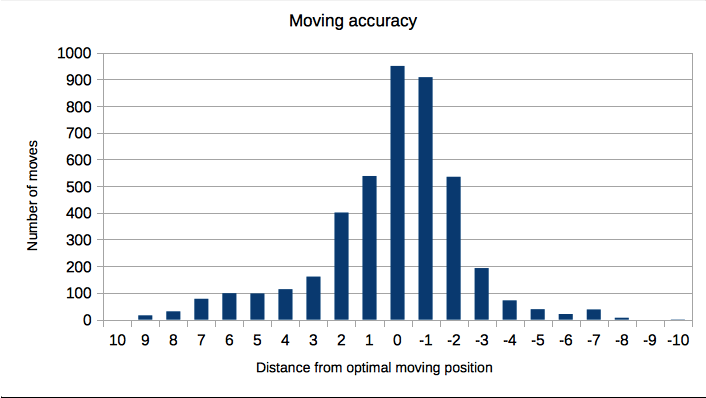
\includegraphics[width=1\textwidth]{movingaccuracy.png}}
           \caption{Moving accuracy: the majority of moving operations are in conformity with the optimal rate of gain}
\end{figure}

From the result displayed by the above chart, we can see that the majority of moving operations is performed at the right time which matches expectations put forth by the Information Foraging Theory. 

\begin{figure} [!ht] 
	\centering
           \makebox[\textwidth][c]{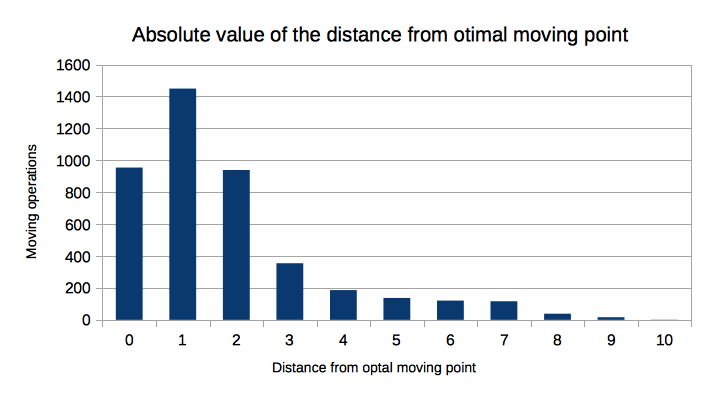
\includegraphics[width=0.9\textwidth]{absolute.png}}
           
           \caption{Absolute moving accuracy: in total, users are stop digging either one layer above or one layer below the optimal point}
           \label{fig:absolute}
\end{figure}

Chart~\ref{fig:absolute} however, shows that if we consider the absolute value of the the difference between the layer number at which the user should have moved minus the value at which they did actually move, we notice that the majority of users moves either one layer below or one layer above the optimal moving point.

\section{Moving accuracy and scanning equipment}

Because the scanning equipment influences the amount of layers the users can see cues (gold flecks) as well as the accuracy of those cues, we investigated the link between the user's scanning equipment in relation to the optimal moving position (optimal gain). 

\begin{figure} [!ht] 
	\centering
           \makebox[\textwidth][c]{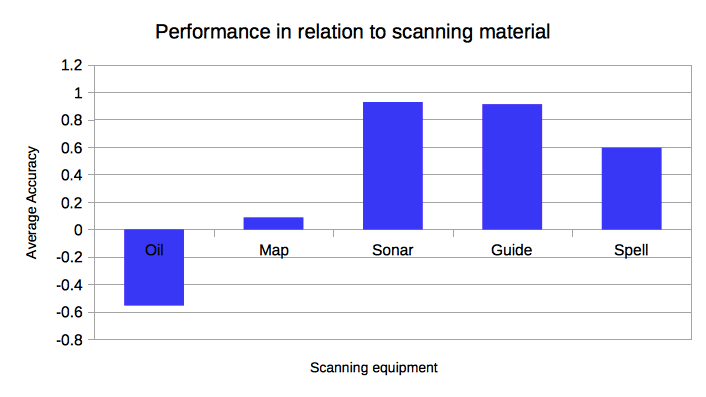
\includegraphics[width=0.9\textwidth]{scan.png}}
           \caption{Scanning equipment seems to have an effect on the ability of the users to predict the optimal moving point}
	  \label{fig:scan}
\end{figure}

From \ref{fig:scan} it seems that, on average, when users are using the Oil Lamp they tend to stop too early, while when they are using the Map, they are very close to an optimal moving point. However, with the next three items, users seem to go too far. 

\section{Moving accuracy and dig  and moving costs}

Another important parameter users have to consider while playing is the cost in time of each digging operation. The more the operation costs, the least amount of digs they will be able to perform. By buying better items, users can decrease this cost and modify their performance. In the chart \ref{fig:digc} we can see the average accuracy in relation to the moving cost (and hence the tool equipped).

\begin{figure} [!ht] 
	\centering
           \makebox[\textwidth][c]{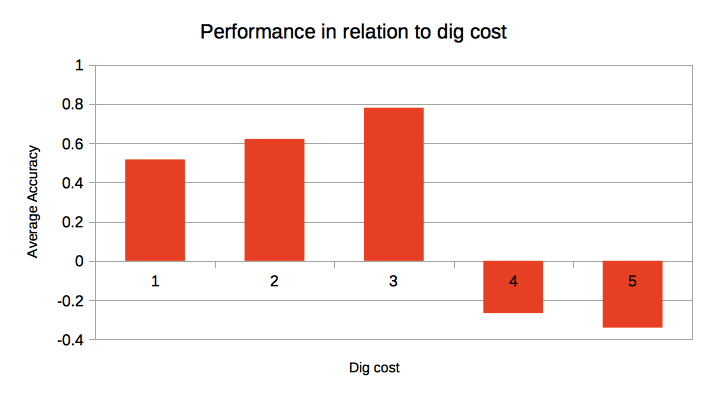
\includegraphics[width=0.9\textwidth]{digc.png}}
           \caption{User performance in relation to dig cost}
	  \label{fig:digc}
\end{figure}

This is quite interesting since it seems that, while the cost of digging is higher, users tend to play it safe and stop digging earlier. However, as the cost of digging decreases, users seem to be more daring and start moving too late instead albeit in a decreasing fashion with each improved item. 

The relationship between moving cost and and moving accuracy, on the other hand doesn't seem too interesting. In fact, as we can see from chart \ref{fig:movec} user behaviour doesn't seem to match any significant pattern in relation to moving cost.

\begin{figure} [!ht] 
	\centering
           \makebox[\textwidth][c]{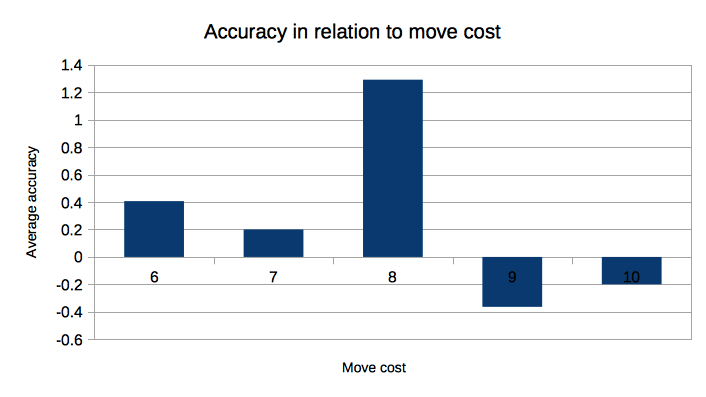
\includegraphics[width=0.9\textwidth]{movec.png}}
           \caption{User performance in relation to move cost}
	  \label{fig:movec}
\end{figure}

\section{Discussion of Results}

From the analysis of the gathered data we seem to be able to confirm some of our expectations regarding users' behaviour in an environment that simulates searching behaviour. In Gold Digger we have created a metaphor for searching by designing an environment that in which users have to make the same sort of choices as they would while searching for information. 

First of all, if we consider the total amount of digging operations performed by all the users during the course of the experiment, we see that the highest number of these operations occurs when the difference between the number of the layer where they should have moved and the one of the layer where they did actually move is equal to 0. This suggests that expectations are met with regards to the Information Foraging Theory. Even in an environment in which there is no relation to information retrieval, the user still performs in the same way, adjusting her strategy to maximise her gain. However, if we consider the \textit{absolute} value of the distance from the optimal moving point, the picture seems to change slightly. In this case, in fact, we can see that, out of all the moving operations performed, the ones that were performed the most were the ones that occurred either one layer too early or one layer too late. This said, however, we can still notice that there is a very clear pattern showing at least the \textit{tendence} of users to behave optimally.

The relationship between users' proximity to optimal behaviour and scanning material has been considered in order to investigate whether a greater insight on what a layer of the mine might contain influences user performance. In a normal information retrieval task this would equate to increasing our knowledge of the material we are searching for, thus being able to tell if a piece of information will be useful to us or not. The relationship found was quite interesting. Users seem to be less cautious with they have the Oil Lamp equipped and they can thus see only see the first two layers of an undug mine showing gold flecks. When they acquire the Map, they start to be very close to optimal performance but, while using the last three items, they seem to leave earlier than they should. I believe that this is due to the user's ability to have enough clues as to how much gold a layer will yield while not being very trustworthy of the cues themselves. In fact, from the moment they acquire the Sonar, they seem to start moving closer and closer to optimal behaviour. 

To represent '\textit{enrichment strategies}' (see ~\ref{subsec:OFT}) in Gold Digger, we introduced items that modify digging and moving cost simulating \textit{in-patch} and \textit{between-patch} enrichment strategies respectively. For this reason, it is important to look at the relationship of digging and moving costs with users' accuracy in trying to achieve optimal gain. For what concerns digging cost, our findings are quite interesting. When digging is the most expensive (4 or 5 units of time) users seem to go deeper an overshoot the optimal mark. This might be because they are anxious to find more gold, since if they don't they won't be able to continue mining an they will encounter a game over. However, when digging gets cheaper because of the purchase of new items, users have probably already managed to store a fair amount of gold. For this reason, it is possible that they don't mind moving to early and pay a comparatively higher price for moving. Since they can afford their mistakes they are eager to get to a new mine and start getting more gold. This seems to also be confirmed by a number of users whom reported the game to be more difficult in the earlier stages. Finally, the relationship between moving cost and accuracy doesn't seem to hold interesting relationship.

\section{Future Work}

In the previous section we have seen just some of the relationships we can extract from the data gathered with Gold Digger, but many more can be investigated and highlighted. One example of this would be the accuracy of the players in relation to each of the mines, is there any mine in which users perform better, and if so, why. Another interesting relationship to explore could be the rapport between the number of mines dug and the accuracy of each player, or the number of days it takes for a player to reach her best performance and if this one is maintained. The means to extract and analyse this kind of data have already been implemented in Gold Digger, however, time constraint didn't allow us to explore them all.

To continue on this path, nevertheless we need to consider Gold Digger's game mechanics first, since users' performance and behaviour could be based on the way they experience the game. Using the data already gathered we could fine-tune the yield functions, the item costs and the mine costs in order to make the game more challenging and enhance the possibility of failure, which in turn will bring the users to pay more attention to their actions. Having done this, we would also need to add more rewards for the users, in order to give them something to work for and strive towards. An example of this would be implementing a performance-based star award system, in which users are awarded one out of three stars in relation to their performance. The closer they get to an optimal gain, the more stars they will get. Another way to reward the users and keep them interested would be adding more items or buildings to purchase with their gold. This way they would be able to have an objective to continue digging, other than simply being at the top of the leaderboards. 

It has been pointed out by some players that some graphical and UI changes could be made to enhance Gold Digger's game play. For example, some user inquired about the presence of sound effects to be played while digging or moving, as well as a background theme. One player suggested that something other than gold should be found and that there should be the possibility to lose gold because of accidents while digging. While on the one hand some of these suggestions are very good and interesting, some of them don't seem to be completely in line with the nature of Gold Digger as an experimental platform for searching behaviour. Losing gold while digging, for instance would not fit in with the theories we set out to test.

\section{Reflection}

Throughout the whole project, from design, to development, to deployment, I had the chance to be faced with many challenges. I am very happy to have had this chance as every one of them thought me invaluable skills that I very much wanted to acquire. Learning to program in Python and using it to code a whole web app in Django from start to finish was a very intense but fulfilling experience.

I believe that the first challenge I was faced with was designing the yield functions for each of the mines. Because they had to be predictable but yet contain a certain degree of randomness, I had to review my knowledge of mathematics and find the right equations to match and then translate them into Django. While doing this, I also helped myself with an online graphing tool to visualize each of them.

Another big challenge, for me, has been the development of the look and feel of Gold Digger. I was very much set to give it an 8-bit retro-looking style. Both because I like it and because it is popular at the moment in the gaming  world. To this end I had to craft my own graphics and find the ones I couldn't make myself. Making them fit together in every page was also part of the challenge, but I think the final version is quite close to my initial vision.

Finally, the biggest challenge has probably been managing the interplay of many different technologies, especially in the game screens where there's so much going on. On one hand Django tags need to display the appropriate content when the page is loaded the first time, on the other AJAX script will have to modify it without "breaking" it, all the wile accessing the appropriate views. 

Overall, I must say I am very proud of this achievement and I am grateful to have had the opportunity to learn so much.
%%%%%%%%%%%%%%%%%%%%%%%%%%%%%%%%%%%%%%%%%%%%%%%%%%%%%%%%%%%%%%%%%%%



%%%%%%%%%%%%%%%%%%%%%%%%%%%%%%%%%%%%%%%%%%%%%%%%%%%%%%%%%%%%%%%%%%%

\appendix % first appendix
%%%%%%%%%%%%%%%%%%%%%%%%%%%%%%%%%%%%%%%%%%%%%%%%%%%%%%%%%%%%%%%%%%%
\chapter{First appendix}
\label{app:firstapp}

\section{Section of first appendix}

%%%%%%%%%%%%%%%%%%%%%%%%%%%%%%%%%%%%%%%%%%%%%%%%%%%%%%%%%%%%%%%%%%%
\chapter{Second appendix}

%%%%%%%%%%%%%%%%%%%%%%%%%%%%%%%%%%%%%%%%%%%%%%%%%%%%%%%%%%%%%%%%%%%
% it is fine to change the bibliography style if you want

\bibliographystyle{plain}
\bibliography{mproj}
\nocite{*}
\end{document}
